%  LaTeX support: latex@mdpi.com 
%  In case you need support, please attach all files that are necessary for compiling as well as the log file, and specify the details of your LaTeX setup (which operating system and LaTeX version / tools you are using).

%=================================================================
\documentclass[sensors,article,submit,moreauthors,pdftex]{Definitions/mdpi} 
% \documentclass[preprint,article,submit,moreauthors,pdftex]{Definitions/mdpi} 

% If you would like to post an early version of this manuscript as a preprint, you may use preprint as the journal and change 'submit' to 'accept'. The document class line would be, e.g., \documentclass[preprints,article,accept,moreauthors,pdftex]{mdpi}. This is especially recommended for submission to arXiv, where line numbers should be removed before posting. For preprints.org, the editorial staff will make this change immediately prior to posting.

%--------------------
% Class Options:
%--------------------
%----------
% journal
%----------
% Choose between the following MDPI journals:
% acoustics, actuators, addictions, admsci, aerospace, agriculture, agriengineering, agronomy, algorithms, animals, antibiotics, antibodies, antioxidants, applsci, arts, asc, asi, atmosphere, atoms, axioms, batteries, bdcc, behavsci , beverages, bioengineering, biology, biomedicines, biomimetics, biomolecules, biosensors, brainsci , buildings, cancers, carbon , catalysts, cells, ceramics, challenges, chemengineering, chemistry, chemosensors, children, cleantechnol, climate, clockssleep, cmd, coatings, colloids, computation, computers, condensedmatter, cosmetics, cryptography, crystals, dairy, data, dentistry, designs , diagnostics, diseases, diversity, drones, econometrics, economies, education, ejihpe, electrochem, electronics, energies, entropy, environments, epigenomes, est, fermentation, fibers, fire, fishes, fluids, foods, forecasting, forests, fractalfract, futureinternet, futurephys, galaxies, games, gastrointestdisord, gels, genealogy, genes, geohazards, geosciences, geriatrics, hazardousmatters, healthcare, heritage, highthroughput, horticulturae, humanities, hydrology, ijerph, ijfs, ijgi, ijms, ijns, ijtpp, informatics, information, infrastructures, inorganics, insects, instruments, inventions, iot, j, jcdd, jcm, jcp, jcs, jdb, jfb, jfmk, jimaging, jintelligence, jlpea, jmmp, jmse, jnt, jof, joitmc, jpm, jrfm, jsan, land, languages, laws, life, literature, logistics, lubricants, machines, magnetochemistry, make, marinedrugs, materials, mathematics, mca, medicina, medicines, medsci, membranes, metabolites, metals, microarrays, micromachines, microorganisms, minerals, modelling, molbank, molecules, mps, mti, nanomaterials, ncrna, neuroglia, nitrogen, notspecified, nutrients, ohbm, optics, particles, pathogens, pharmaceuticals, pharmaceutics, pharmacy, philosophies, photonics, physics, plants, plasma, polymers, polysaccharides, preprints , proceedings, processes, proteomes, psych, publications, quantumrep, quaternary, qubs, reactions, recycling, religions, remotesensing, reports, resources, risks, robotics, safety, sci, scipharm, sensors, separations, sexes, signals, sinusitis, smartcities, sna, societies, socsci, soilsystems, sports, standards, stats, surfaces, surgeries, sustainability, symmetry, systems, technologies, test, toxics, toxins, tropicalmed, universe, urbansci, vaccines, vehicles, vetsci, vibration, viruses, vision, water, wem, wevj

%---------
% article
%---------
% The default type of manuscript is "article", but can be replaced by: 
% abstract, addendum, article, benchmark, book, bookreview, briefreport, casereport, changes, comment, commentary, communication, conceptpaper, conferenceproceedings, correction, conferencereport, expressionofconcern, extendedabstract, meetingreport, creative, datadescriptor, discussion, editorial, essay, erratum, hypothesis, interestingimages, letter, meetingreport, newbookreceived, obituary, opinion, projectreport, reply, retraction, review, perspective, protocol, shortnote, supfile, technicalnote, viewpoint
% supfile = supplementary materials

%----------
% submit
%----------
% The class option "submit" will be changed to "accept" by the Editorial Office when the paper is accepted. This will only make changes to the frontpage (e.g., the logo of the journal will get visible), the headings, and the copyright information. Also, line numbering will be removed. Journal info and pagination for accepted papers will also be assigned by the Editorial Office.

%------------------
% moreauthors
%------------------
% If there is only one author the class option oneauthor should be used. Otherwise use the class option moreauthors.

%---------
% pdftex
%---------
% The option pdftex is for use with pdfLaTeX. If eps figures are used, remove the option pdftex and use LaTeX and dvi2pdf.

%=================================================================
\firstpage{1} 
\makeatletter 
\setcounter{page}{\@firstpage} 
\makeatother
\pubvolume{xx}
\issuenum{1}
\articlenumber{5}
\pubyear{2019}
\copyrightyear{2019}
%\externaleditor{Academic Editor: name}
\history{Received: date; Accepted: date; Published: date}
%\updates{yes} % If there is an update available, un-comment this line

%% MDPI internal command: uncomment if new journal that already uses continuous page numbers 
%\continuouspages{yes}

%------------------------------------------------------------------
% The following line should be uncommented if the LaTeX file is uploaded to arXiv.org
%\pdfoutput=1

%=================================================================
% Add packages and commands here. The following packages are loaded in our class file: fontenc, calc, indentfirst, fancyhdr, graphicx, lastpage, ifthen, lineno, float, amsmath, setspace, enumitem, mathpazo, booktabs, titlesec, etoolbox, amsthm, hyphenat, natbib, hyperref, footmisc, geometry, caption, url, mdframed, tabto, soul, multirow, microtype, tikz
\usepackage{caption}
\usepackage{subcaption}

%=================================================================
%% Please use the following mathematics environments: Theorem, Lemma, Corollary, Proposition, Characterization, Property, Problem, Example, ExamplesandDefinitions, Hypothesis, Remark, Definition, Notation, Assumption
%% For proofs, please use the proof environment (the amsthm package is loaded by the MDPI class).

%=================================================================
% Full title of the paper (Capitalized)
% \Title{Understanding Human Activity Recognition using LSTM Networks for Wearables and Prosthesis}
\Title{Understanding LSTM Network Behaviour for IMU based Human Activity Recognition in Prosthesis and Wearables}

% Author Orchid ID: enter ID or remove command
\newcommand{\orcidauthorA}{0000-0003-3611-4846} % Add \orcidA{} behind the author's name
\newcommand{\orcidauthorB}{0000-0002-4965-0341} % Add \orcidB{} behind the author's name

% Authors, for the paper (add full first names)
% \Author{Frederick Sherratt $^{1,\dagger,\ddagger}$\orcidA{} and Pejman Iravani $^{2,}$*\orcidB{}}
\Author{Frederick Sherratt \orcidA{} and Pejman Iravani *\orcidB{}}
% Authors, for metadata in PDF
\AuthorNames{Frederick Sherratt and Pejman Iravani}

% Affiliations / Addresses (Add [1] after \address if there is only one affiliation.)
% \address{%
% $^{1}$ \quad Affiliation 1; f.w.sherratt@bath.ac.uk\\
% $^{2}$ \quad Affiliation 2; p.iravani@bath.ac.uk}
\address[1]{Department of Mechanical Engineering, University of Bath; f.w.sherratt@bath.ac.uk}
% Contact information of the corresponding author
\corres{Correspondence: e-mail@e-mail.com; Tel.: (optional; include country code; if there are multiple corresponding authors, add author initials) +xx-xxxx-xxx-xxxx (F.L.)}

% Current address and/or shared authorship
% \firstnote{Current address: Affiliation 3} 
% \secondnote{These authors contributed equally to this work.}
% The commands \thirdnote{} till \eighthnote{} are available for further notes

%\simplesumm{} % Simple summary

%\conference{} % An extended version of a conference paper

% Abstract (Do not insert blank lines, i.e. \\) 
\abstract{A single paragraph of about 200 words maximum. For research articles, abstracts should give a pertinent overview of the work. We strongly encourage authors to use the following style of structured abstracts, but without headings: (1) Background: Place the question addressed in a broad context and highlight the purpose of the study; (2) Methods: Describe briefly the main methods or treatments applied; (3) Results: Summarize the article's main findings; and (4) Conclusion: Indicate the main conclusions or interpretations. The abstract should be an objective representation of the article, it must not contain results which are not presented and substantiated in the main text and should not exaggerate the main conclusions.}

% Keywords
\keyword{keyword 1; keyword 2; keyword 3 (list three to ten pertinent keywords specific to the article, yet reasonably common within the subject discipline.)}

% The fields PACS, MSC, and JEL may be left empty or commented out if not applicable
%\PACS{J0101}
%\MSC{}
%\JEL{}

%%%%%%%%%%%%%%%%%%%%%%%%%%%%%%%%%%%%%%%%%%
% Only for the journal Diversity
%\LSID{\url{http://}}

%%%%%%%%%%%%%%%%%%%%%%%%%%%%%%%%%%%%%%%%%%
% Only for the journal Applied Sciences:
%\featuredapplication{Authors are encouraged to provide a concise description of the specific application or a potential application of the work. This section is not mandatory.}
%%%%%%%%%%%%%%%%%%%%%%%%%%%%%%%%%%%%%%%%%%

%%%%%%%%%%%%%%%%%%%%%%%%%%%%%%%%%%%%%%%%%%
% Only for the journal Data:
%\dataset{DOI number or link to the deposited data set in cases where the data set is published or set to be published separately. If the data set is submitted and will be published as a supplement to this paper in the journal Data, this field will be filled by the editors of the journal. In this case, please make sure to submit the data set as a supplement when entering your manuscript into our manuscript editorial system.}

%\datasetlicense{license under which the data set is made available (CC0, CC-BY, CC-BY-SA, CC-BY-NC, etc.)}

%%%%%%%%%%%%%%%%%%%%%%%%%%%%%%%%%%%%%%%%%%
% Only for the journal Toxins
%\keycontribution{The breakthroughs or highlights of the manuscript. Authors can write one or two sentences to describe the most important part of the paper.}

%\setcounter{secnumdepth}{4}
%%%%%%%%%%%%%%%%%%%%%%%%%%%%%%%%%%%%%%%%%%
\begin{document}
%%%%%%%%%%%%%%%%%%%%%%%%%%%%%%%%%%%%%%%%%%

%%%%%%%%%%%%%%%%%%%%%%%%%%%%%%%%%%%%%%%%%%
\section{Introduction}
% Generic introduction to prosthesis and the problems users face
For the able bodied it is taken for granted that during locomotion both legs will act in unison adapting to the environment and activity without thought; for lower limb amputees this ability is lost. Amputees suffer from poor gait due to muscle imbalances and significant compensatory mechanism are required to adapt to the lost of muscle and joints\cite{Silverman2008}. This results in musculoskeletal problems, increased energetic cost of locomotion and an increased risk of falling\cite{Herr2012, Piazza2017, McDonald2018}. The next generation of prosthesis aim to replicate the lost power generating muscles functionality in an attempt to improve gait. In order for the prosthetic to work in synergy with the user it must recognise the users intent, therefore a system of Human Activity Recognition (HAR) is required.

% What existing solutions are there.
There are already commercially available prosthesis that actively adapt to the users intent such as Ottobock's Enpower BiOM\cite{Enpower}, Blatchford's ElanIC\cite{ElanIC} and \"Ossur's Proprio Foot\cite{Proprio}. Bone of the three provide more that basic functionality such as maintaining dorsiflexion during swing to increase toe clearance and adjusting ankle resistance based on terrain. Only the BiOM ankle provides a powered ankle to assist in push off. These features rely on user selection or heuristics control strategies.

% Problems\Research gaps
Machine Learning (ML) offers the ability to significantly increase the sophistication of such systems though understand of a wide range of activities and personalisation to individual characteristics without specialist intervention\cite{Labarriere2020}. This is where the current state of the art is. Sequential ML networks appear to a good fit for this problem but little is know of there underlying behaviour. For a medical device such as a prosthetic both a detailed knowledge of internal network operation and high levels of accuracy are required. 

% How we going about answering research gap/question
In this paper we explore in detail the operation and performance of Long Short Term Memory (LSTM) networks for HAR using both seen and novel users. Data from able-bodied participants is used as a substitute for amputee data as it allows for a much larger and varied data set while minimising risk to subjects. This is then used to investigate the internal operation on a simplified LSTM network. The effect of hyper-parameters on the generalisation performance of a full complexity LSTM network are then investigated. Finally changes to the model are investigated to try and improve its performance for novel users. The major contributions of this work are as follows:
% What are the major contributions of this paper
\begin{enumerate}
\item Methodology for and collection of large self-supervised wearable Inertial Measurement Units (IMU) data set of human activity data in a natural environments.
\item Provide an insight into the behaviour of an LSTM HAR model and why that limits it's generalisation (method for visually understanding lstm).
\item Investigation of model modification to reduce model confusion around the transition between locomotion modes.
\item Demonstrate a need for personalisation techniques
\end{enumerate}

The remainder of this paper is organized as follows; Section \ref{sec:human_gait_cycle} presents theory on the human gait cycle and it's relevance to HAR. In section \ref{sec:lstm_therory} ML in HAR. the theory of LSTMs and relevant literature is presented. Sections \ref{sec:data_collection} and \ref{sec:app} present the methodology for data collection. Section \ref{sec:simplified_model} includes the methodology and results of analysis for the internal operation of a simplified LSTM HAR network. Section \ref{sec:full_complexity} contains the results of analysis of hyper-parameter sensitivities of a full complexity HAR LSTM network. Section \ref{sec:improving_perfromance} contains work on improving the models performance for novel users. Finally Sections \ref{sec:discussion} and \ref{sec:conclusion} contain discussion and conclusions.




%%%%%%%%%%%%%%%%%%%%%%%%%%%%%%%%%%%%%%%%%%%%%%%%%%%%%%%%%%%%%%%%%%%%%%
% This section talks about the human gait cycle and how it varies between different activities and why different locomotion modes are required.
\section{HAR in the Human Gait Cycle}
\label{sec:human_gait_cycle}
Human gait is a cyclic process that can be delineated by key event. A gait cycle is defined by two successive Initial Contact (IC) event, the point at which part of the foot contacts the ground, of the same limb. As this is normally the heel, it is often refereed to as Heel Strike (HS). Conversely the point when the foot leaves the ground is referred to as Toe Off (TO). These two events are used to subdivide the gait into two phases; stance - when the foot is on the ground, and swing when not. A diagram showing these events and there place in the gait cycles is shown in Figure \ref{fig:gait_cycle}.

\begin{figure}[!htb]
    \centering
    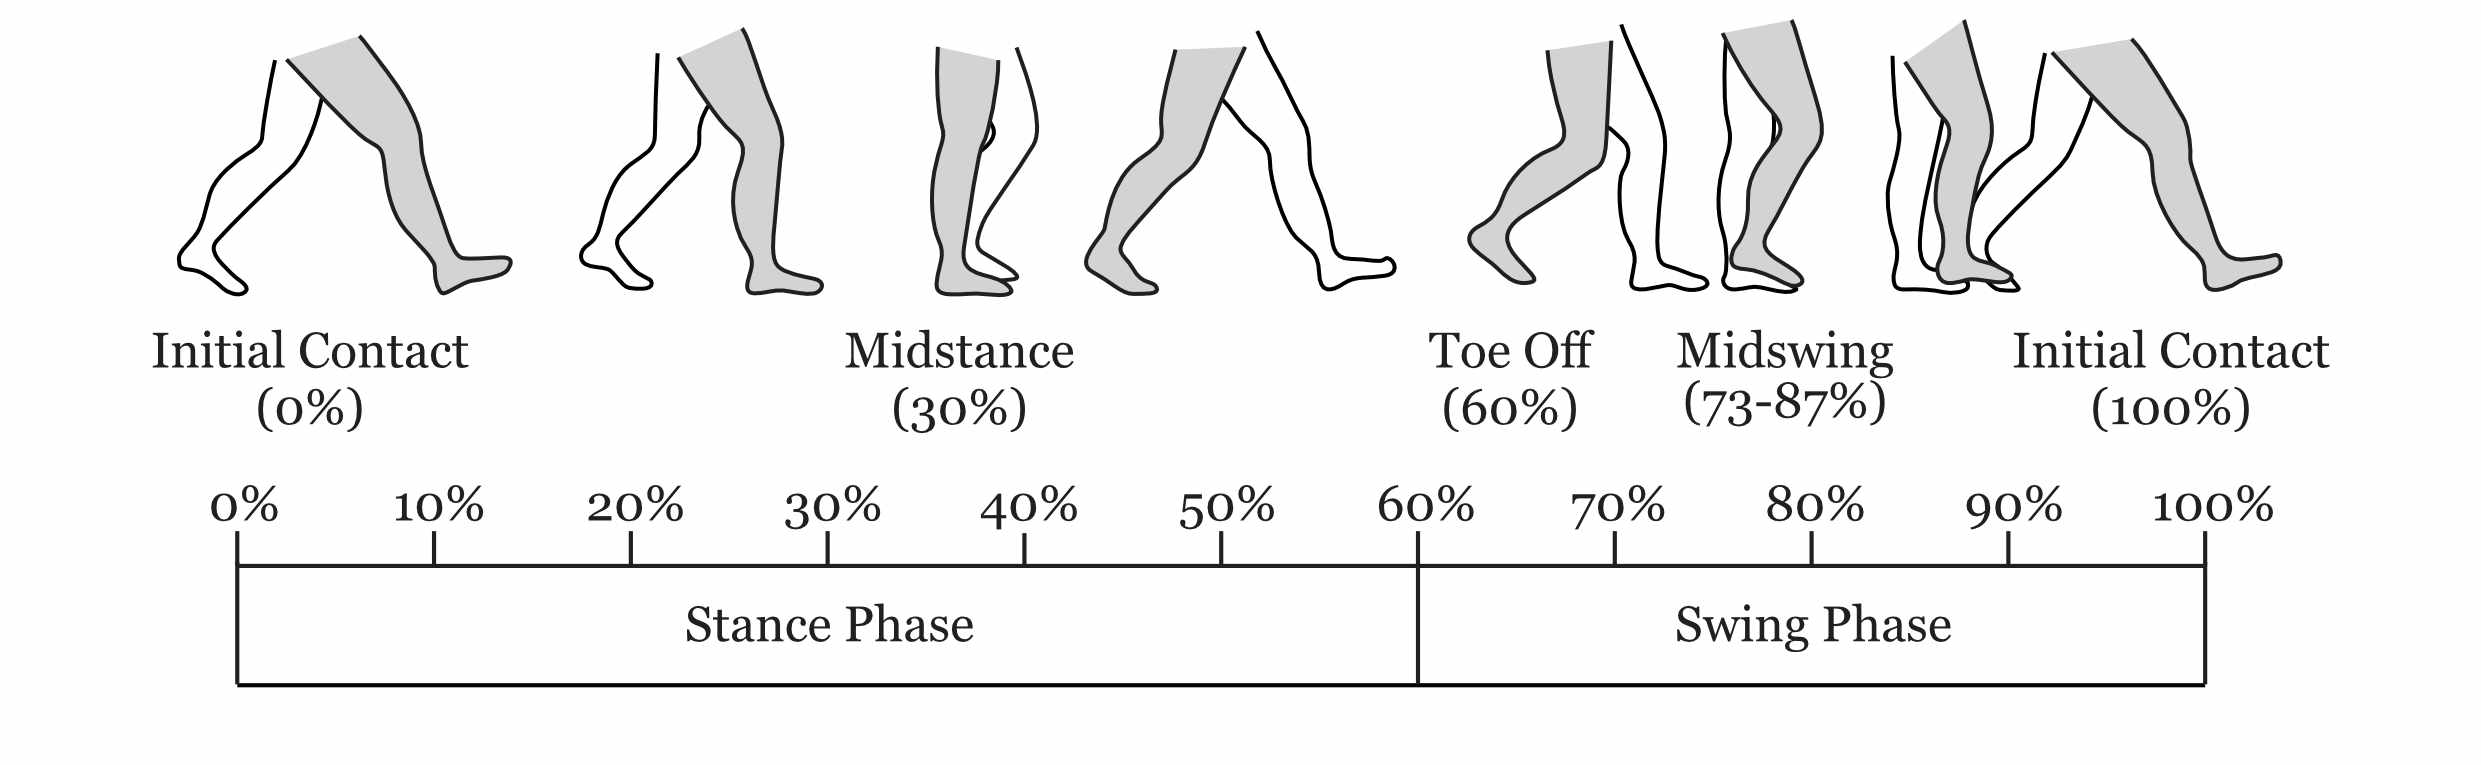
\includegraphics[width=\textwidth]{Figures/Gait_Cycle.jpg}
    \caption{Human Gait Cycle during level walking, adapter from \cite{humanGaitCycle2016}}
    \label{fig:gait_cycle}
\end{figure}

It has been shown that gait events can be established from only extreme of the shank angular velocity in the sagittal plane\footnote{The sagittal plane divides the body into left and right, so rotation in this plane is forward and backward motion of the shank} using a technique originally presented by Sabatini et al\cite{Sabatini2005}. IC/HS was found to line up with the minima following peak swing velocity and TO was identified as the half way point between the zero crossing and the minima before peak swing. Figure \ref{fig:y-gyro-hs-to} shows the gyroscope trace of a sensor attached to a subjects shank with the locations of the calculated TO and IC events indicated.

\begin{figure}[!htb]
    \centering
    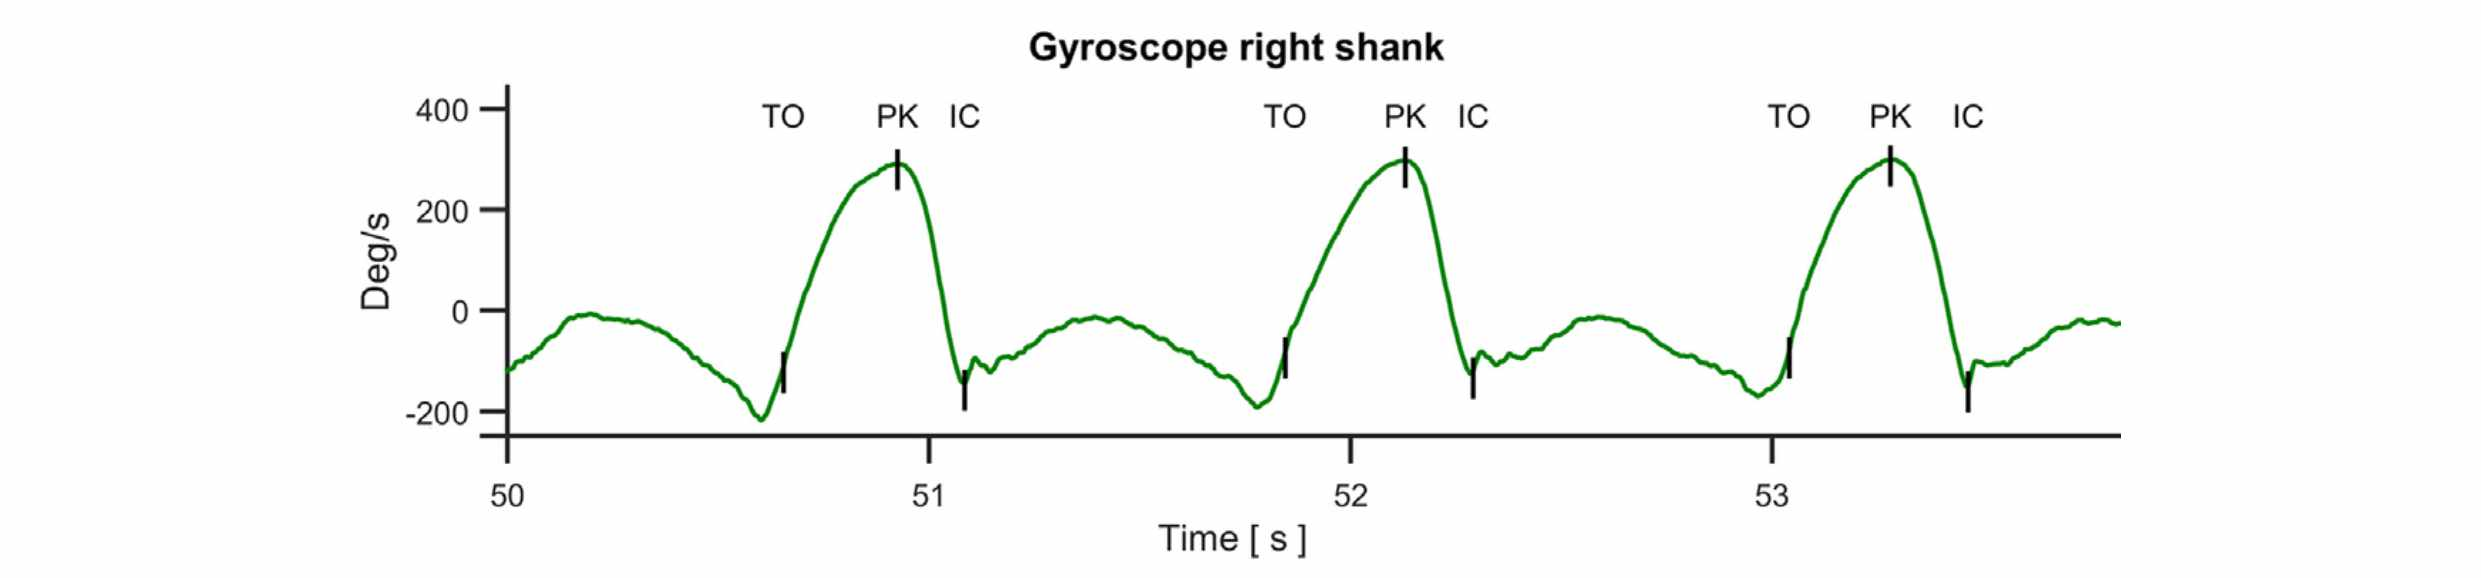
\includegraphics[width=\textwidth]{Figures/gyro_trace_hs.jpg}
    \caption{Gait events extracted from the sagittal plane gyroscope signal, adapter from \cite{Sabatini2005}. IC - Initial Contact, PK - Peak Swing, TO - Toe Off}
    \label{fig:y-gyro-hs-to}
\end{figure}

% How does HAR relate to the human gait?
The action of the leg varies depending on the activity. To accommodate this powered prosthesis will require multiple locomotive mode to achieve the different timing and power requirement. Therefore automated recognition of the users intentions and subsequent selection of the corresponding locomotive mode will be crucial to the performance of device.\cite{Tucker2015, Windrich2016, Zhang2015} In order for amputees to have confidence in the device its activity recognition must be timely, accurate and consistent and able adaptive to account for the individual gait characteristics.\cite{Pedroli2019, Sinha2011, Ponce2016}

For the current generation of prosthetic devices this is achieved though hand tuned heuristic. These methods identify and associate changing properties in sensor data with different activities. For example Coley et al noted that the variation in shank sagittal plane rotational velocity that occurs from stairs. It was noted that during early stance there is an increase in rotational velocity during stair descent and a decrease during stair ascent when compared to level walking.\cite{Coley2005}. The current state of the art in HAR uses Machine learning methods to accomplish activity recognition, these techniques will be discussed further in the next section.




%%%%%%%%%%%%%%%%%%%%%%%%%%%%%%%%%%%%%%%%%%%%%%%%%%%%%%%%%%%%%%%%%%%%%%%%
% Introduce ML in HAR and benefits over heuristics; RNN and LSTM theory; what have other people done in the area
\section{LSTM Networks for HAR} 
\label{sec:lstm_therory}
HAR for active prosthesis has conventionally been achieved through heuristic methods with hand picked features and manual-tuned for each individual \cite{Maqbool2017, Xu2018}. This approach is favoured by the commercial market due to safety and regulatory concerns\cite{Fluit2020}. However the tuning of these controllers is time consuming and requires a highly skilled prosthetist. In the current state of the art HAR techniques, the focus has been on the use of Machine Learning techniques to automate the process of feature selection and output classification and personalisation\cite{Labarriere2020}.

Many different machine learning techniques have been investigated including, Support Vector Machines, Hidden Markov Models and Convolution Neural Network with success\cite{Labarriere2020}. As sensor data from human gait is temporal the best architecture for solving this will be one that can take into account the sequential nature of the input data. The Recurrent Neural Network (RNN) is a ML architecture suited to handling sequential data. It contains both forward and horizontal hidden states connections. The hidden state connections allow a representation of previous the inputs to be passed along the sequence. Figure \ref{fig:rnn_structure} shows the unfolded structure of a recurrent network. It can be seen that the activation of each cell is dependent on both it's inputs and the internal hidden states of the previous time steps.

\begin{figure}[!hbt]
    \centering
    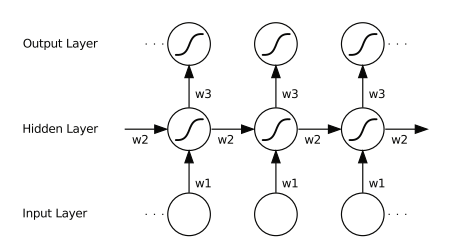
\includegraphics[width=0.6\textwidth]{Figures/lstm/rnn_structure.png}
    \caption{Unfolded Recurrent Network}
    \label{fig:rnn_structure}
\end{figure}

Each timestep in the network can contain a number of hidden states or units. This is better represented by Equation \ref{eqn:rnn_activation} showing the activation input. $\mathbf{a}$ is formed from the bias vector $\mathbf{b}$ plus the sum of input vectors $\mathbf{x}$ and previous hidden states $\mathbf{h}$, times there weight matrices $\mathbf{W}$ and $\mathbf{U}$ for hidden-to-hidden state input-to-hidden state connections respectively.\cite{Goodfellow2015} The shape of a RNN network is often described by its timesteps x units for example 128x6.

\begin{equation}
    \mathbf{a}^{(t)} = \mathbf{b} + \mathbf{Wh}^{(t-1)} + \mathbf{Ux}^{(t)}
    \label{eqn:rnn_activation}
\end{equation}

%What problems exist with them 
RNNs have been shown to produce good results in some sequential task but there application is limited by difficulty in training. The primarily difficulty is the vanishing/exploding gradient problem. During gradient based training methods repeated multiplication by values that are not near 1 along long dependency chains result in values that either vanish or explode. A vanishing gradients makes it difficult to know which direction the parameters should move to improve the cost function, while exploding gradients can make learning unstable. Non-gradient based training have been tried although to limited success. \cite{Graves2012, Goodfellow2015}

% LSTM
The Long Short Term Memory (LSTM) architecture solve the vanishing gradient problem by adding mechanisms for regulating information allowing it to be retained for long periods. Created by Hochreiter and Schmidhuber in 1997\cite{Hochreiter1997} the LSTM is an RNN style architecture that includes additional gaits to control information flow between cells, see Figure \ref{fig:lstm_unit}. Information flowing along the cell state can be modulated by the input and forget gate structures with the final output of a filtered version of the cell state based on context from the inputs.\cite{Olah2015}  

\begin{figure}[!htb]
    \centering
    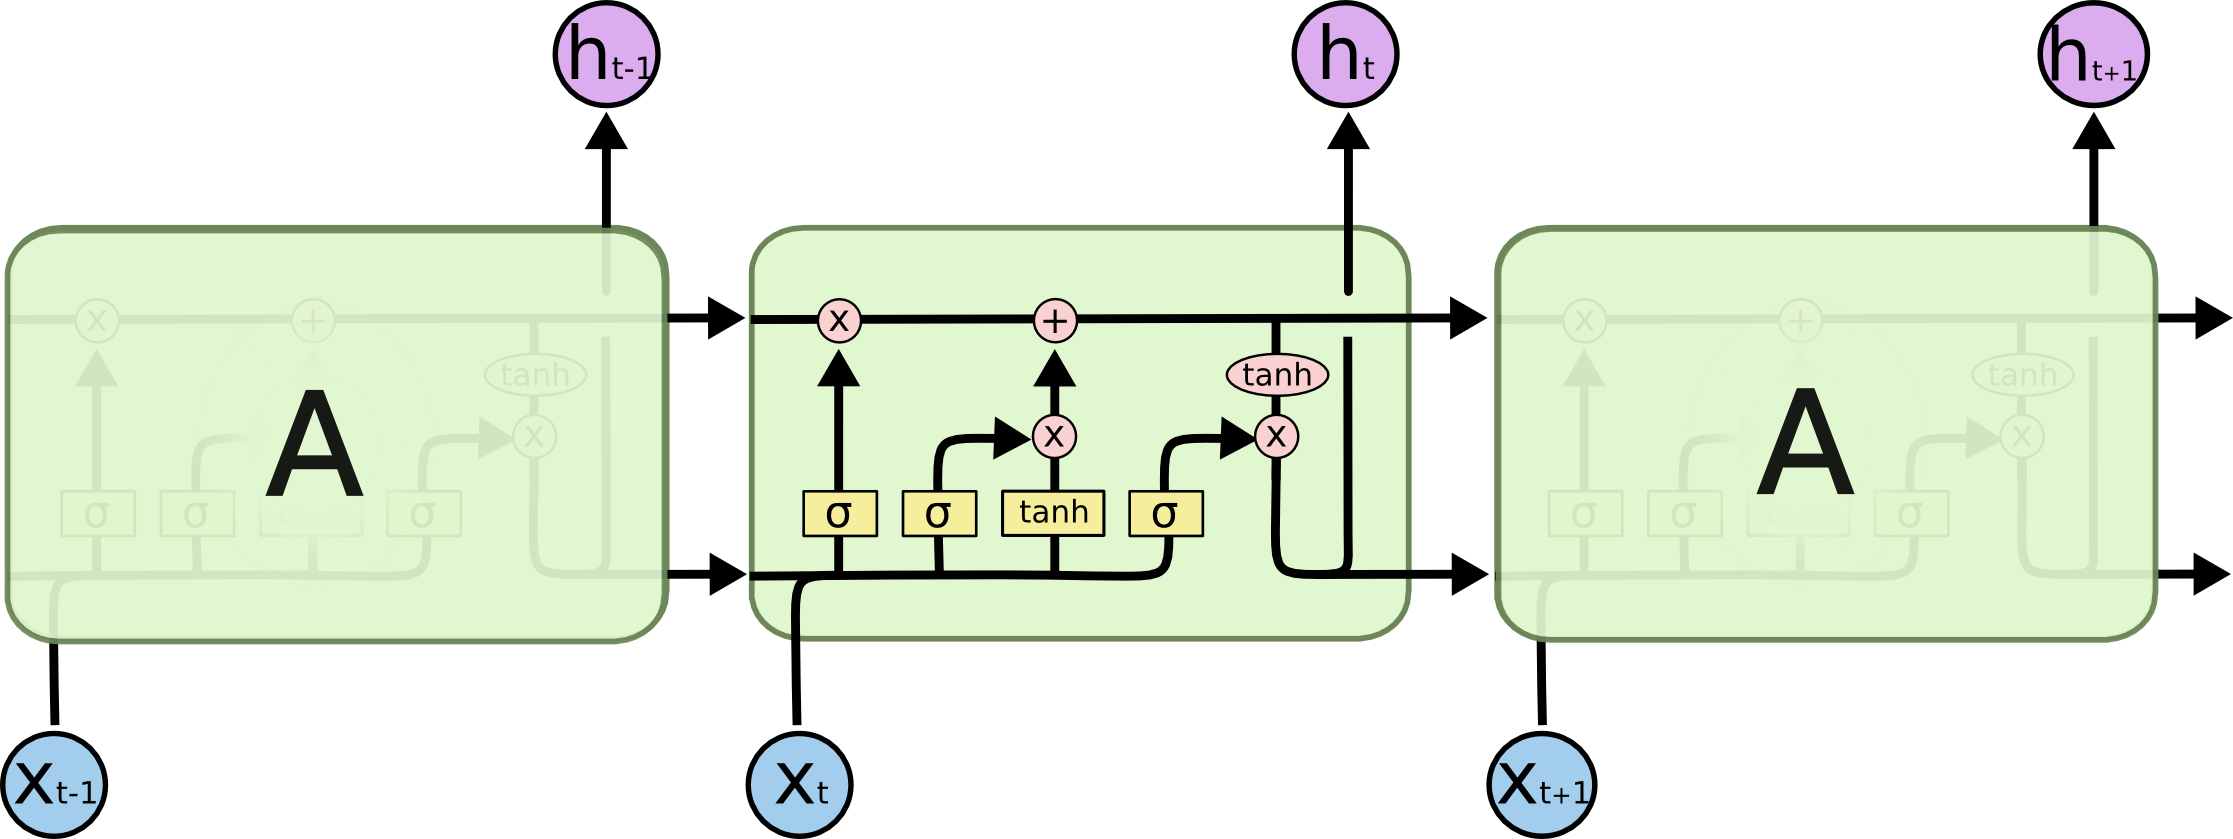
\includegraphics[width=0.7\textwidth]{Figures/lstm/LSTM-chain.png}
    \caption{LSTM unit with input and output connections \cite{Olah2015}}
    \label{fig:lstm_unit}
\end{figure}


%%%%%% Lit Review
%In literature most LSTM model are structured as in Figure \ref{fig:full_lstm_model}. 

\subsection{Related Works}
%What are common structures of an LSTM network? Should add more on what HAR means for Gait cycle recognition, what are the actions / states / etc/ Relate this to what you mentioned on safety and user confidence
In HAR tasks LSTMs have been demonstrated to provide exceptional performance\cite{Murad2017} although very little work has been done investigating this in the context of prosthesis\cite{Fluit2020}.

Labarri\`ere et al has produced a systematic review of the machine learning methods used in activity recognition for assistive device\cite{Labarriere2020}. Labbrrie\`ere found the most common activities to are Walking, Stair Ascent, Stair Descent, Ramp Ascent, Ramp Descent.

LSTM exo-skeleton\cite{Wang2018}, identifies sitting down, standing up, level-ground walking, ascending stairs, and descending stair activities based on angle information from hip, knee and ankle joints. Uses a deep LSTM architecture to select modes.

% Ben-Yue Su et al present work investigating intent prediction for trans-tibial amputees using IMU data fed into a CNN network\cite{Su2019} The 10 able-bodied and 1 trans-tibial amputee were asked to perform short walks traversing a short stair case and ramp as with a level surface either side. The able bodied subjects wore a hands-free crutch. Three IMUs were attached to the thigh, shank and ankle of the “healthy” leg.

%The raw sensor data is fed as an input vector into the first LSTM layer of n units. The hidden state vector from this layer is then fed into subsequent LSTM layers. The last output of the final LSTM layer is passed into a dense classification layer. Some authors have used a fully connected final layer using the output from every cell, termed later fusion.

Murad and Pyun presented a paper investigating human activity recognition using Deep LSTM network\cite{Murad2017}. They train their network on common ADL datasets presenting their performance in comparison to other work on these datasets. The network they used took the raw IMU data as it's input then interpreted the data using four LSTM layers before a late fusion dense layer and a softmax classifer were user to produce a class output, see Figure \ref{fig:murad_lst_network_structure}. Performance was very impressive achieving between 92 \& 97\% accuracy and an improvement on the presented previous classification attempts using of CNN, SVM and others networks.

\begin{figure}[!htb]
    \centering
    \includegraphics[width=0.7\textwidth]{example-image-a}
    \caption{Murad et al raw IMU LSTM Network Structure}
    \label{fig:murad_lst_network_structure}
\end{figure}

A different network configuration used for each data set and there are large differences between the datasets which makes for difficult comparisons between experiments, but it demonstrates that their method is more widely applicable. The model accuracy is also based purely on the validation data, the validation data is a random 20\% of the source data, so sufficient separation between training and validation data is not guaranteed. In the compared work a mixture of evaluation techniques are used, most commonly k-fold cross-validation techniques. With test data selected by leaving out participants [2, 3, 4]. As such it is not clear that a direct comparison can be made to demonstrate LSTMs superiority.

% \cite{Yu2018}

Dehghani et al investigate the metrics used to evaluate the performance of classifiers in regard to there performance to previously unseen data presented using k-fold cross-validation methods\cite{Dehghani2019}. The papers found implement various forms of k-fold validation but none using LSTM use a subject based cross-validation. Instead, they either leave out individual windows \cite{Murad2017, Wang2020}<TK> or, when multiple data sets are recorded for participants, individual recordings \cite{Ordonez2016}<TK>. Dehghani found that this overestimates performance by 10-16\%. Studies that have left individuals out found accuracies closer of 86.7\% \cite{Zhao2018}. The reason for the poor generalisation when presented with a novel user has not been investigated.


A short summary of previous work section to be added.

%LSTM have been shown to achieve high-levels of accuracy but understanding of the internal mechanisms by which they achieve this is limited. They have also only been tested on data collected in controlled conditions.
% Lots of people have tried lots of different techniques but not LSTM - also nothing about new users
% LSTM seems to work really well in HAR challenges
% Although it's not obvious why and seems to struggle with novel users



%%%%%%%%%%%%%%%%%%%%%%%%%%%%%%%%%%%%%%%%%%%%%%%%%%%%%%%%%%%%%%%%
\section{Data Collection}
\label{sec:data_collection}
There are several commonly used data sets for able-bodied activity recognition. The OPPORTUNITY activity recognition dataset\cite{roggan2010} contains 18 activity classes for Activities of Daily Living (ADL) such as opening/closing doors and drinking from a cup. Each subject wore seven 6-axis IMUs and 12 3-axis accelerometers while they preformed the prescribed actions. The UCI-HAD dataset\cite{Anguita2013} recorded subject performing six activities; walking, stair ascent, stair descent, sitting, standing and laying, while wearing waist mounted smart phone with on board Magnetic, Angular Rate and Gravity (MARG) sensors. Both of these data sets were recorded in controlled conditions so do not capture any variation in activity that may occur due to the environment. Sztyler and Stuckenschmidt collected data from 15 subjects performing eight activities while wearing six wearable sensors. Recording took place in the same natural environments for each activity, however only steady state activities were capture not the transition between them.\cite{Sztyler2017} 

% Aim of data collection
Due to limitation in the identified data sets a new set of data is required. The aim of this data set was to record natural locomotion in an unstructured environments, capturing both steady state and also the transition between activities across different environments from a wide range of subjects. Collection of large quantities of data from amputees is very challenging so instead able-boded subjects will be used. Able-bodied subjects will have a less varied gait than amputees but this can be countered by a far larger population size.

Subject were provided with instructions on how to use the sensing equipment and then allowed to record as they wished. The following activities were selected, Walking (W), Stair Ascent (SA), Stair Descent (SD), Ramp Ascent (RA), Ramp Descent (RD) and Stopped (S). These were identified as commonly investigated and required no equipment or skill to perform\cite{Labarriere2020}.

% Sensor selection and location
Non-invasive wearable sensors, such as Inertial Measurement Units, are an appealing choice for developing such a system. IMU give fast update rate, 100s of Hz, are extremely non-invasive (small with minimal mounting constraints), low cost and reasonable accuracy. They have been Widely used in the field, all of the latest generation powered prosthetic knees investigated by Fluit et al contained IMUs\cite{Fluit2020}.

% Which sensors did we use and why
A wearable IMU produced by Movesense was used to collect activity data. The device contains a 9 axis MARG sensor and a Bluetooth Low Energy (BLE) radio in a small 10g package. The sensor housing contains a snap connectors allowing it to be clipped on attachment hardware and a variety of mounting hardware is available off the shelf. The sensor is user-programmable allowing customised behaviour, in this case it was setup to stream IMU data at 100Hz over a BLE connection to a custom app running on an android smart phone. Further details of the app are presented in Section \ref{sec:app}.

Five sensors were attached to each participant in the following locations. On the inside of ankle using an elastic Velcro strap, on each hip using a clothes/belt clip and across the chest using a heart rate strap. The location of the sensors was selected to give a wide covering of body movements while providing easy, secure and non-invasive attachment to minimise discomfort and disruption to natural movement. Figure \ref{fig:movesense_sensors} shows a subject wearing the five sensors.

\begin{figure}[!hbt]
    \centering
    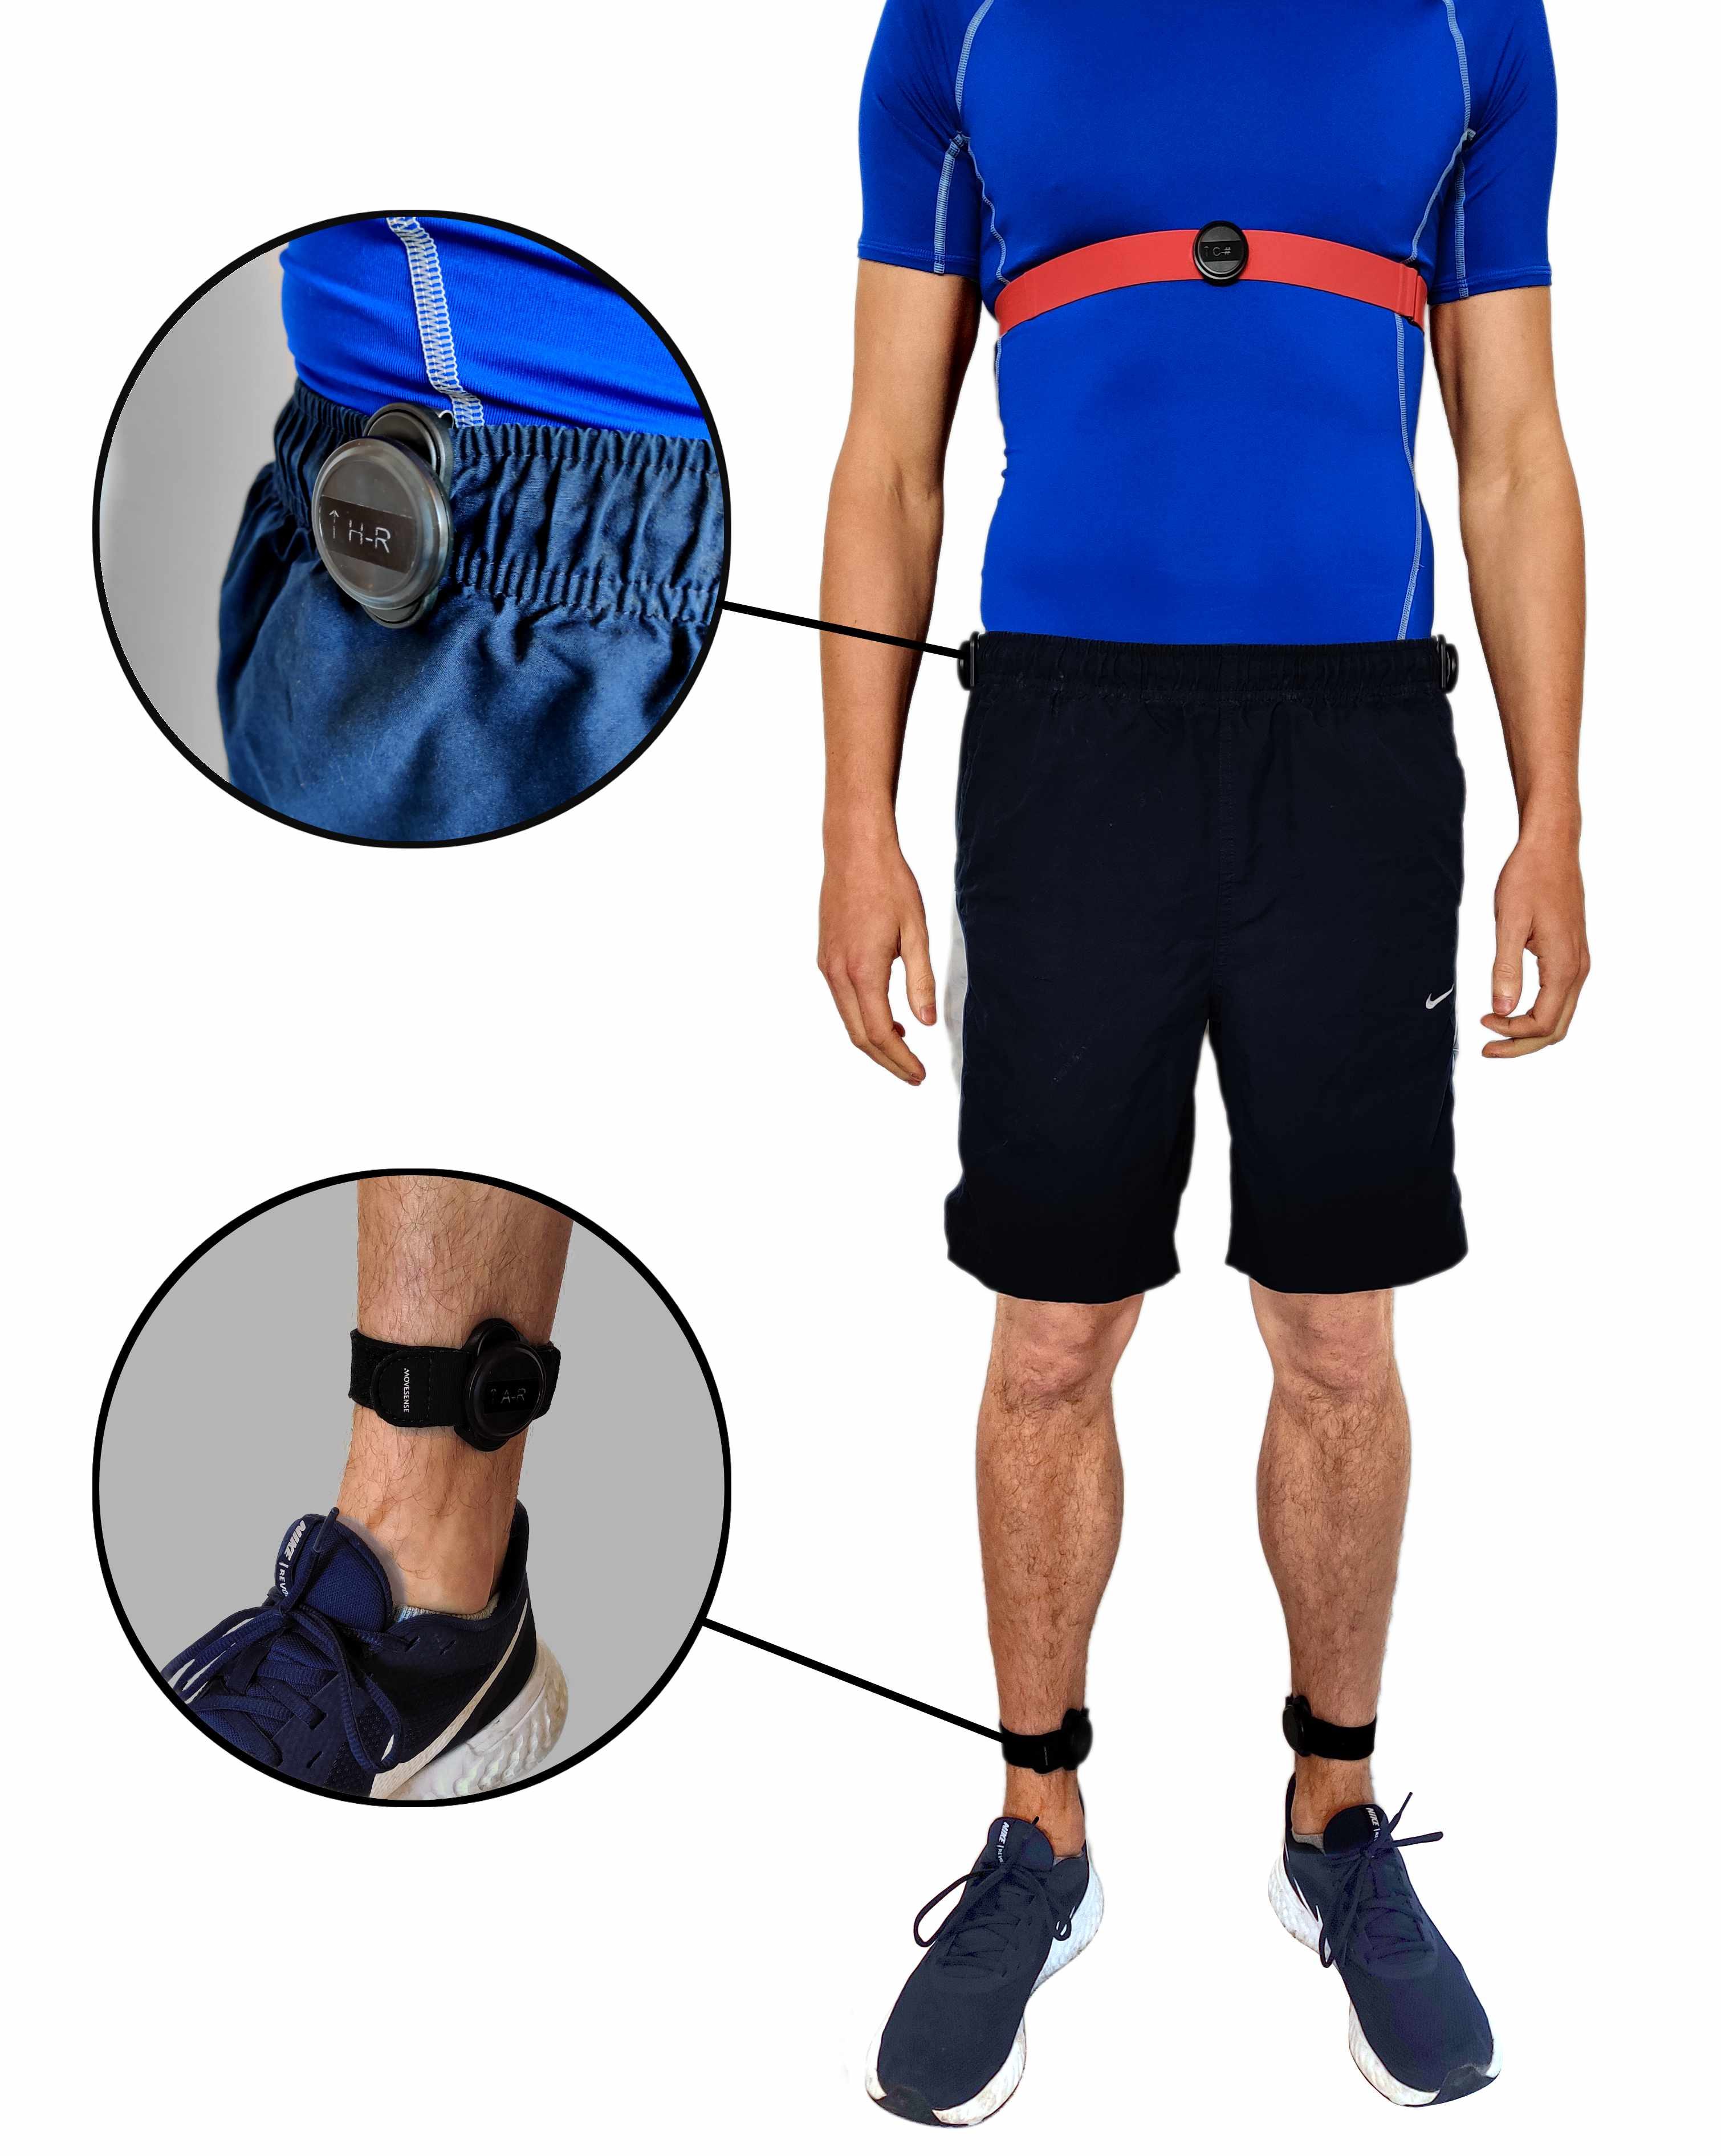
\includegraphics[height=220px]{Figures/movesense/sensor_locations.jpg}
    % \captionsetup{justification=centering}
    \caption{Subject wearing the Movesense IMU sensors on both ankles, hips and the chest}
    \label{fig:movesense_sensors}
\end{figure}

% Participant instructions
Twenty-two Participants of a wide variety of age, gender and physique were chosen to give a broad data set. Participants were instructed to walk around a varied environment with the sensor on while labeling their activities. No further instructions on how the activities should be conducted were provided. A total of 268 minutes of data was collected which includes 1170 transitions between activities. Table \ref{tab:data_collected_summary} contains a summary of the data collected.

% Dataset Statistics
\begin{table}[!hbt]
    \centering
    \caption{Quantity of data collected for each activity}
    \label{tab:data_collected_summary}
    \begin{tabular}{cccc}
        \textbf{Activity} & \textbf{Samples} & \textbf{Time (minutes)} & \textbf{Number of Steps} \\
         \hline
         Walking & 1075211 & 179 & 9438 \\
         Stair Ascent & 139922 & 23 & 1286 \\
         Stair Descent & 122379 & 20 & 1280 \\ 
         Ramp Ascent & 73328 & 12 & 656 \\
         Ramp Descent & 79436 & 13 & 754 \\
         Stop & 121027 & 20 & - \\
         \hline
         \textbf{Total} & 1611303 & 268 & 13414
    \end{tabular}
\end{table}




% Android app
%%%%%%%%%%%%%%%%%%%%%%%%%%%%%%%%%%%%%%%%%%%%%%%%%%%%%%%%%%%%%%%%%%%%%%
\section{Custom App and Data Processing}
\label{sec:app}
To record data from the sensors, a custom android app was created. This formed a BLE connection to each device and saved the streamed data. During recording a series of buttons at the bottom of the screen could be used for real-time labelling of activities. Once recording had finished the subject was presented with a upload screen allowing meta data to be added. The file could then be shared anonymously with the researchers using Google's Firebase cloud services. A screen shot of the app in recording mode is shown in Figure \ref{fig:data_collection_diagrams}.

\begin{figure}[!hbt]
    \centering
    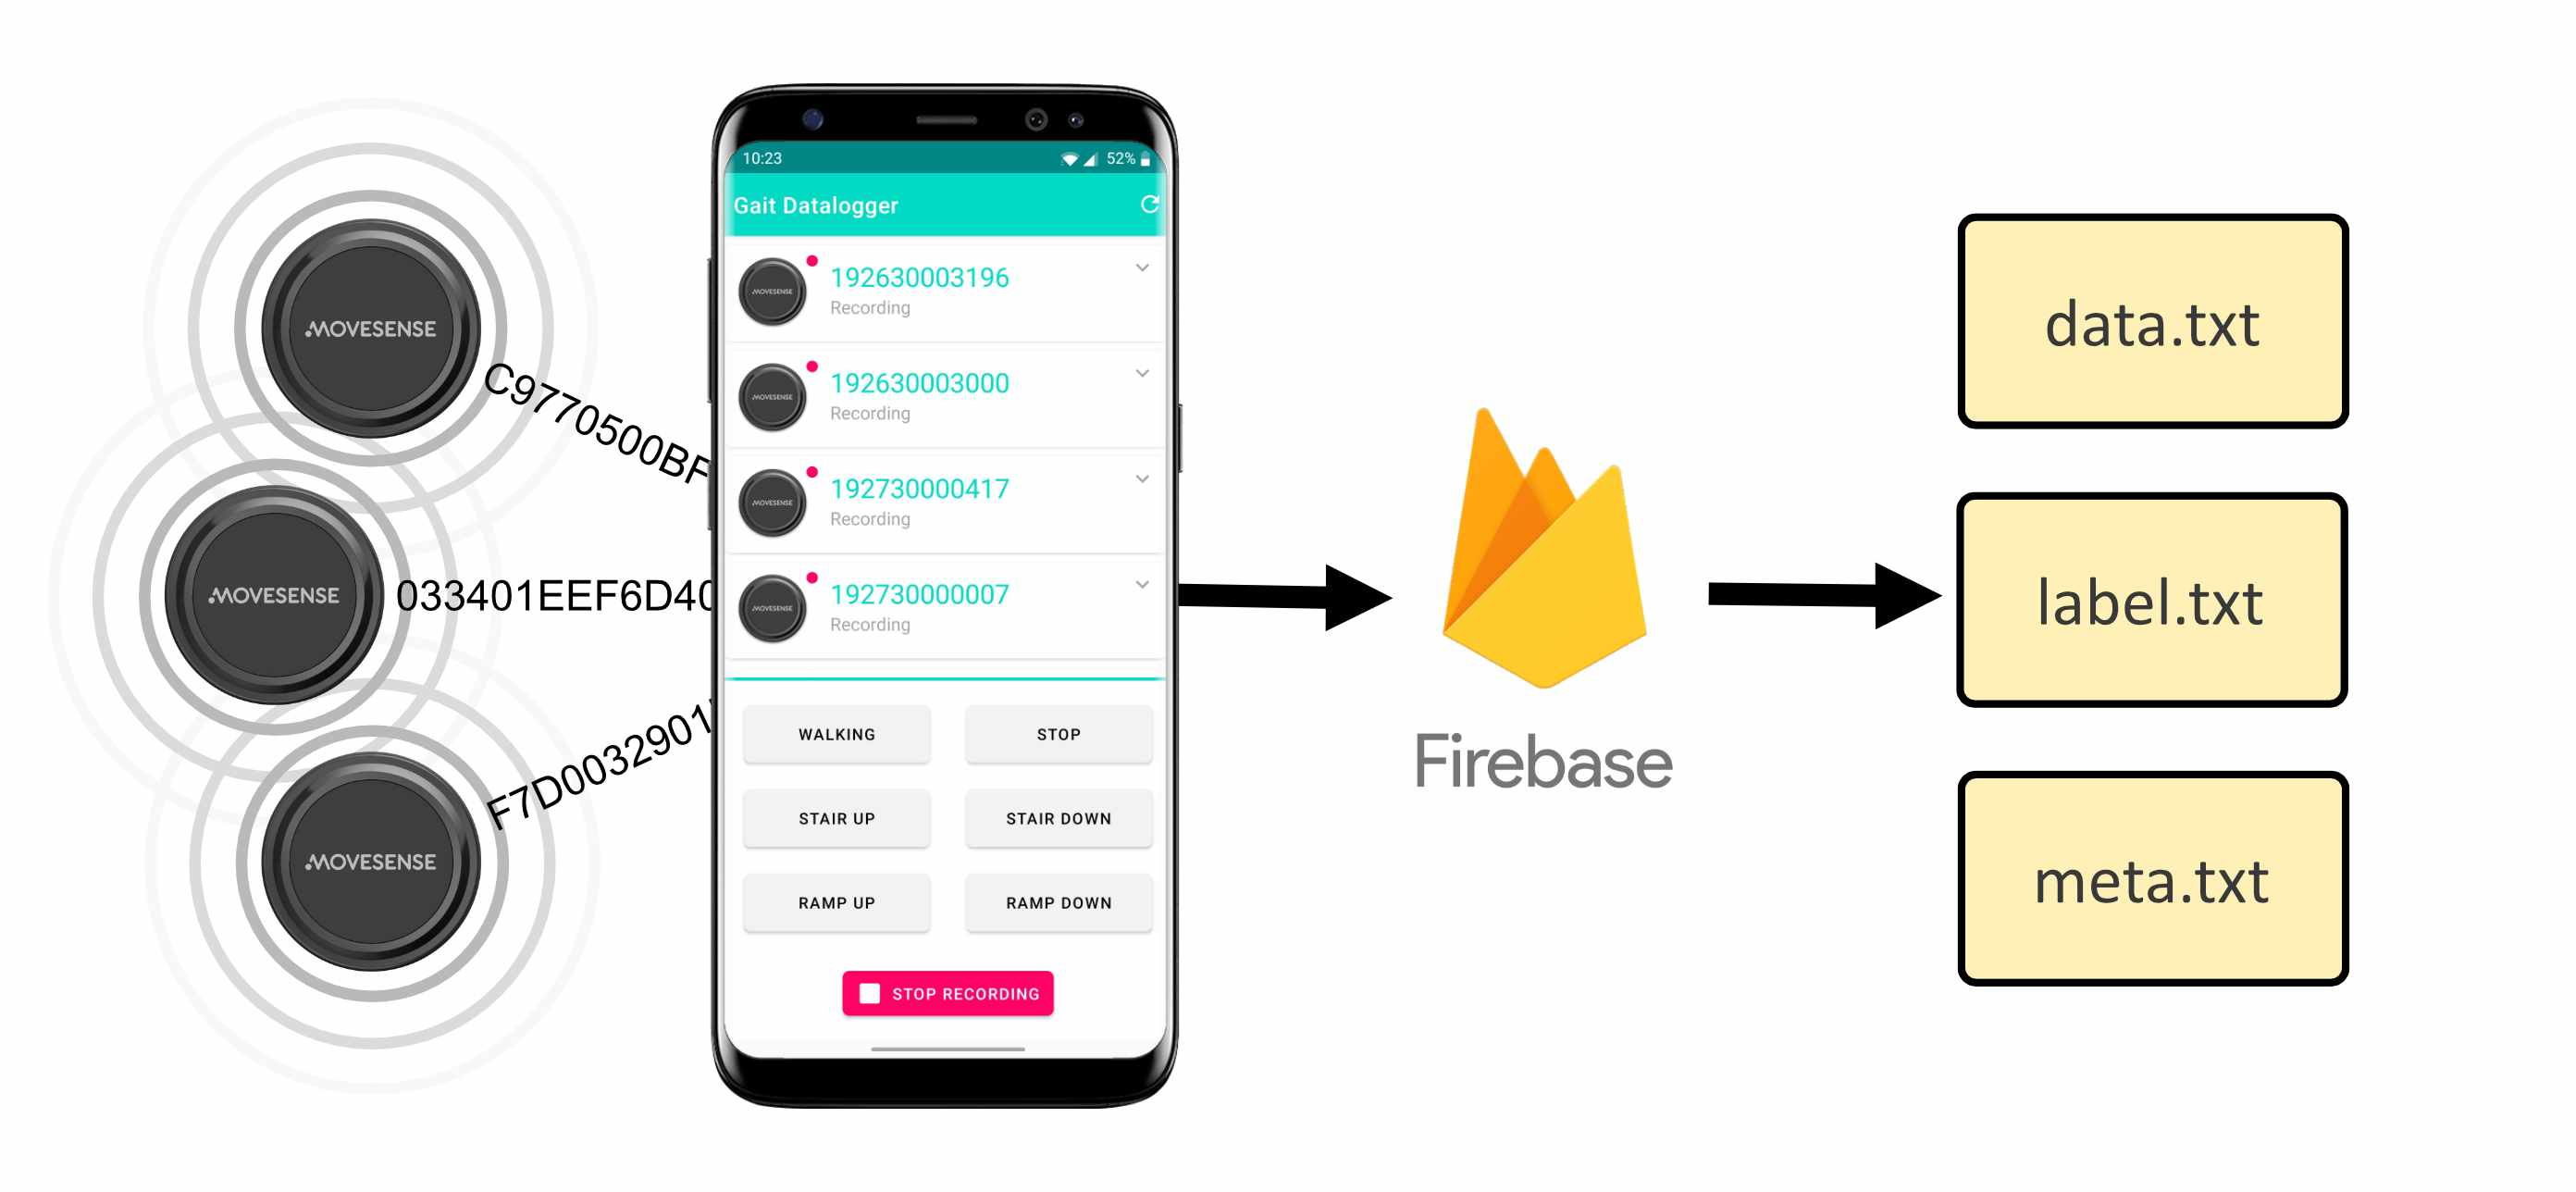
\includegraphics[width=\textwidth]{Figures/movesense/sensor_collection.jpg}
    \caption{Custom Android app with connected sensors and illustration of Firebase upload system}
    \label{subfig:data_collection}
    \label{fig:data_collection_diagrams}
\end{figure}

% Data post-processing
To convert the raw saved data to a form that Tensorflow could import a processing pipeline was developed in Matlab 2019b. The pipeline consisted of decoding, re-sampling, time alignment, normalisation, and exporting. The raw data is saved as transmitted by the sensors so needed to be converted from compressed fixed-point to a floating-point representation. The data was then re-sampled, to compensate for the difference between the internal sensor clocks, using the smartphone clock as a common reference. Finally it was normalised so that for each recording every individual sensor channel had a standard deviation of one and a mean of zero before exporting to a \textit{.csv} file. A flow diagram of this process is shown if Figure \ref{fig:data_processing}.

\begin{figure}[!hbt]
    \centering
    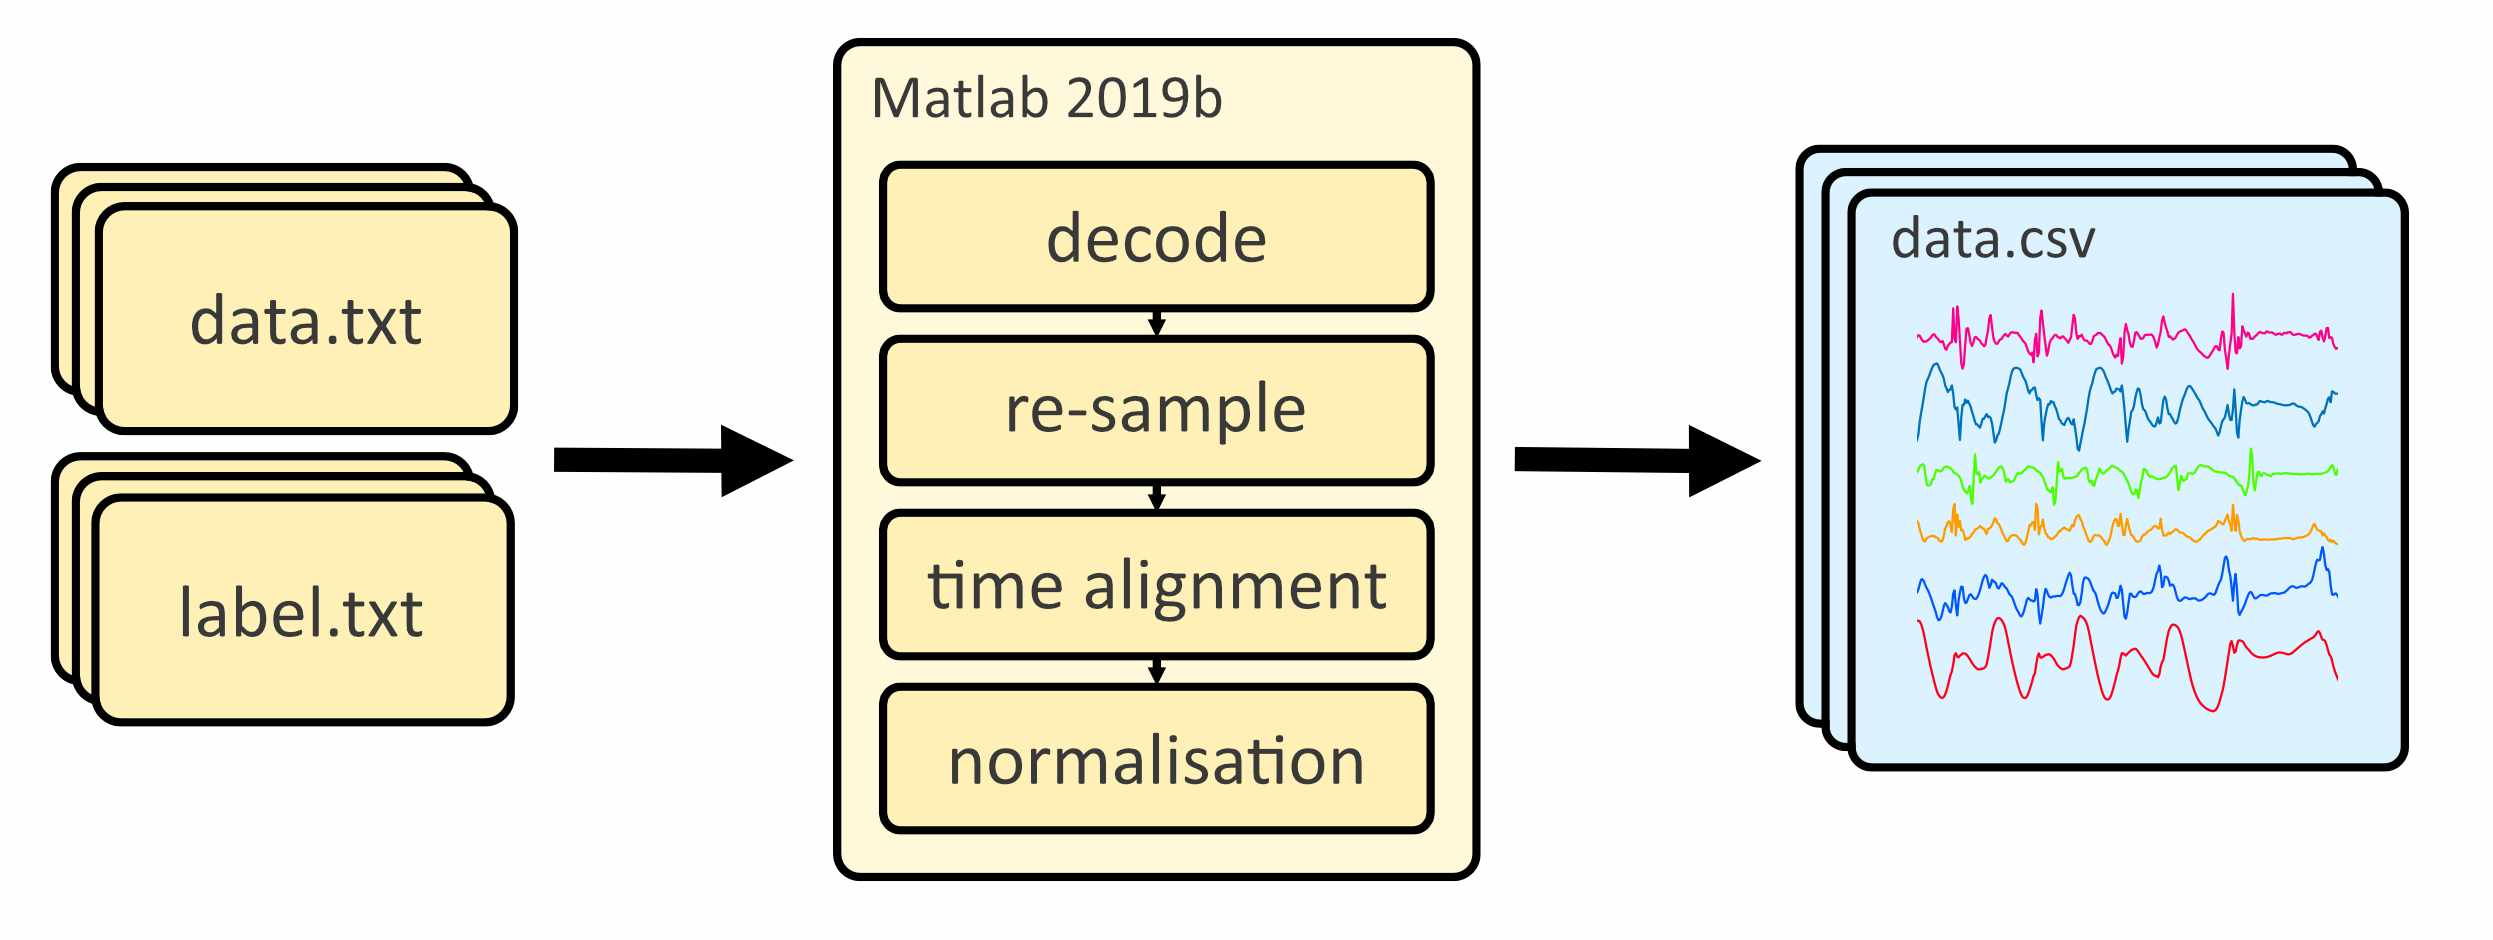
\includegraphics[width=0.8\textwidth]{Figures/movesense/data_processing.jpg}
    \caption{Raw data input and pre-processing flow diagram}
    \label{fig:data_processing}
\end{figure}

% Data axis system
The following axis system will be used when presenting and analysing the results. The axes uses a right hand, front left up convention. $x$ is forward towards the front of the body, $y$ toward the left and $z$ upwards. From this point forward the beginning of the gait cycle, 0\%, will be defined as the peak swing maxima. This leads HS by about 20\%.



%%%%%%%%%%%%%%%%%%%%%%%%%%%%%%%%%%%%%%%%%%
\section{Machine Learning Training}
\label{sec:machine_Learning}
Within this section the methodology for training the machine learning models is presented. All the machine learning models were created using Tensorflow 2.1.0 and Keras. Training undertaken on a computer accelerated using RTX 2060 GPU.

The continuous sensor data was segmented using sliding windows. Between the start of each window a offset of two samples was used. This offset was set empirically to give the model a wide range of data windows position without slowing down learning from an unnecessarily large training set. The output label for each widow was set as the recorded ground truth at the end of the window. Classification labels were presented using one-hot encoding.

The data set is divided into two groups for test and training. The training set is used during the learning process with the test set reserved for evaluating performance of unseen data. The test set is a variation of Leave One Out Cross Validation (LOOXV) where a single subject is excluded from the training set. To reduce computational requirements instead four/five subjects were excluded. The training set contains the remaining subjects, with 30\% of the data used as a validation set. Each model was trained five times with each subject was once. The results were combined to improve statistical certainty. Figure \ref{fig:test_training_split} provides an illustration of how the data is divided between the three classes.

\begin{figure}[!hbt]
    \centering
    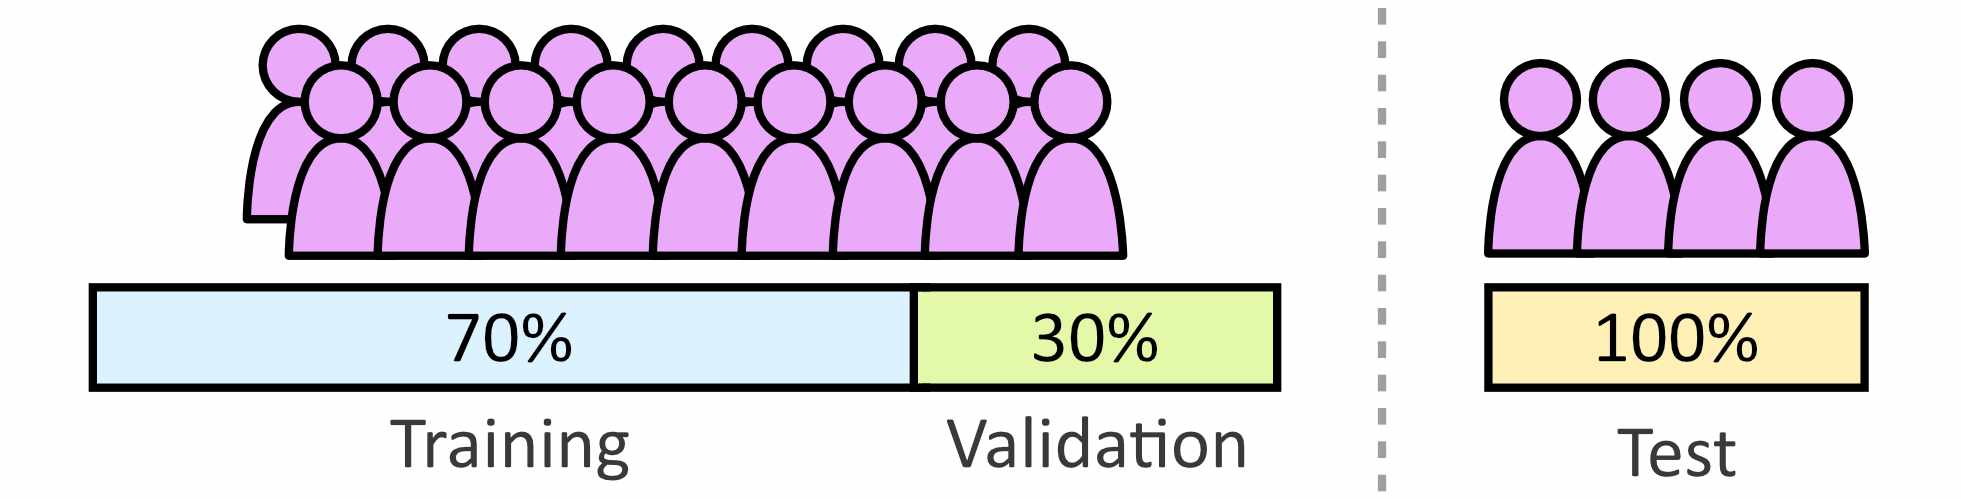
\includegraphics[width=0.7\textwidth]{Figures/test_train_split.jpg}
    \caption{Division of the subject population to form the training, validation and test sets}
    \label{fig:test_training_split}
\end{figure}

To balance the data set both the training and test sets were adjusted so that no class class contains more than 50\% more samples than any another. This re-balancing was undertaken carefully so that during validation splitting the balance was maintained.

To train the models the Adam optimisation algorithm was used, this a very popular algorithm for problems with large data-sets and or parameters\cite{Kingma2015} with initial model weights were set using a Golorot Uniform initialiser. A class weight input was used to bias the training to further balance the class labels. Mini batch sizes of 2000 were used, with early stopping based on validation data cross entropy loss stagnation. Between the output of the LSTM network and dense classifier a dropout of 0.5 was used. According to Srivastava et al this is a close to optimal for a wide range of networks and tasks\cite{Srivastava2014}. Analysis of dropout rates confirmed this.




%%%%%%%%%%%%%%%%%%%%%%%%%%%%%%%%%%%%%%%%%%%%%%%%%%%%%%%%%%%%%%%%%%%%%%%
% Simplified model
\section{Simplified LSTM}
\label{sec:simplified_model}
%Introductory paragraph - Needs an intro explaining we are going to start simple, to show what are the characteristics of LSTM and move the the more complex networks
An understanding of the behaviour of a LSTM can be gained from matching inputs to changes in hidden state. For a full complexity model this is too complicated due to fully connected steps between units making following the path of information extremely challenging. To enable information gained from inputs to be easily traced a single path for it to flow is required. To achieve this a simplified model is required. 

\subsection{Methodology}
% Simplified model - plotting of hidden state
Figure \ref{fig:simplfied_lstm_model} shows the simplified model that will be used for the behavioural analysis. A single unit wide network is used with the final hidden state value passed to a dense classification layer with a ReLU activation. As desired the simplified model provides only one path form information to flow. Logits were used to ensure no scaling occurs along the network. To extract the hidden state for all LSTM units. The weights and biases of the LSTM layer were extracted and copying into a new model with an outputs of the full hidden state sequence.

\begin{figure}[!htb]
    \centering
    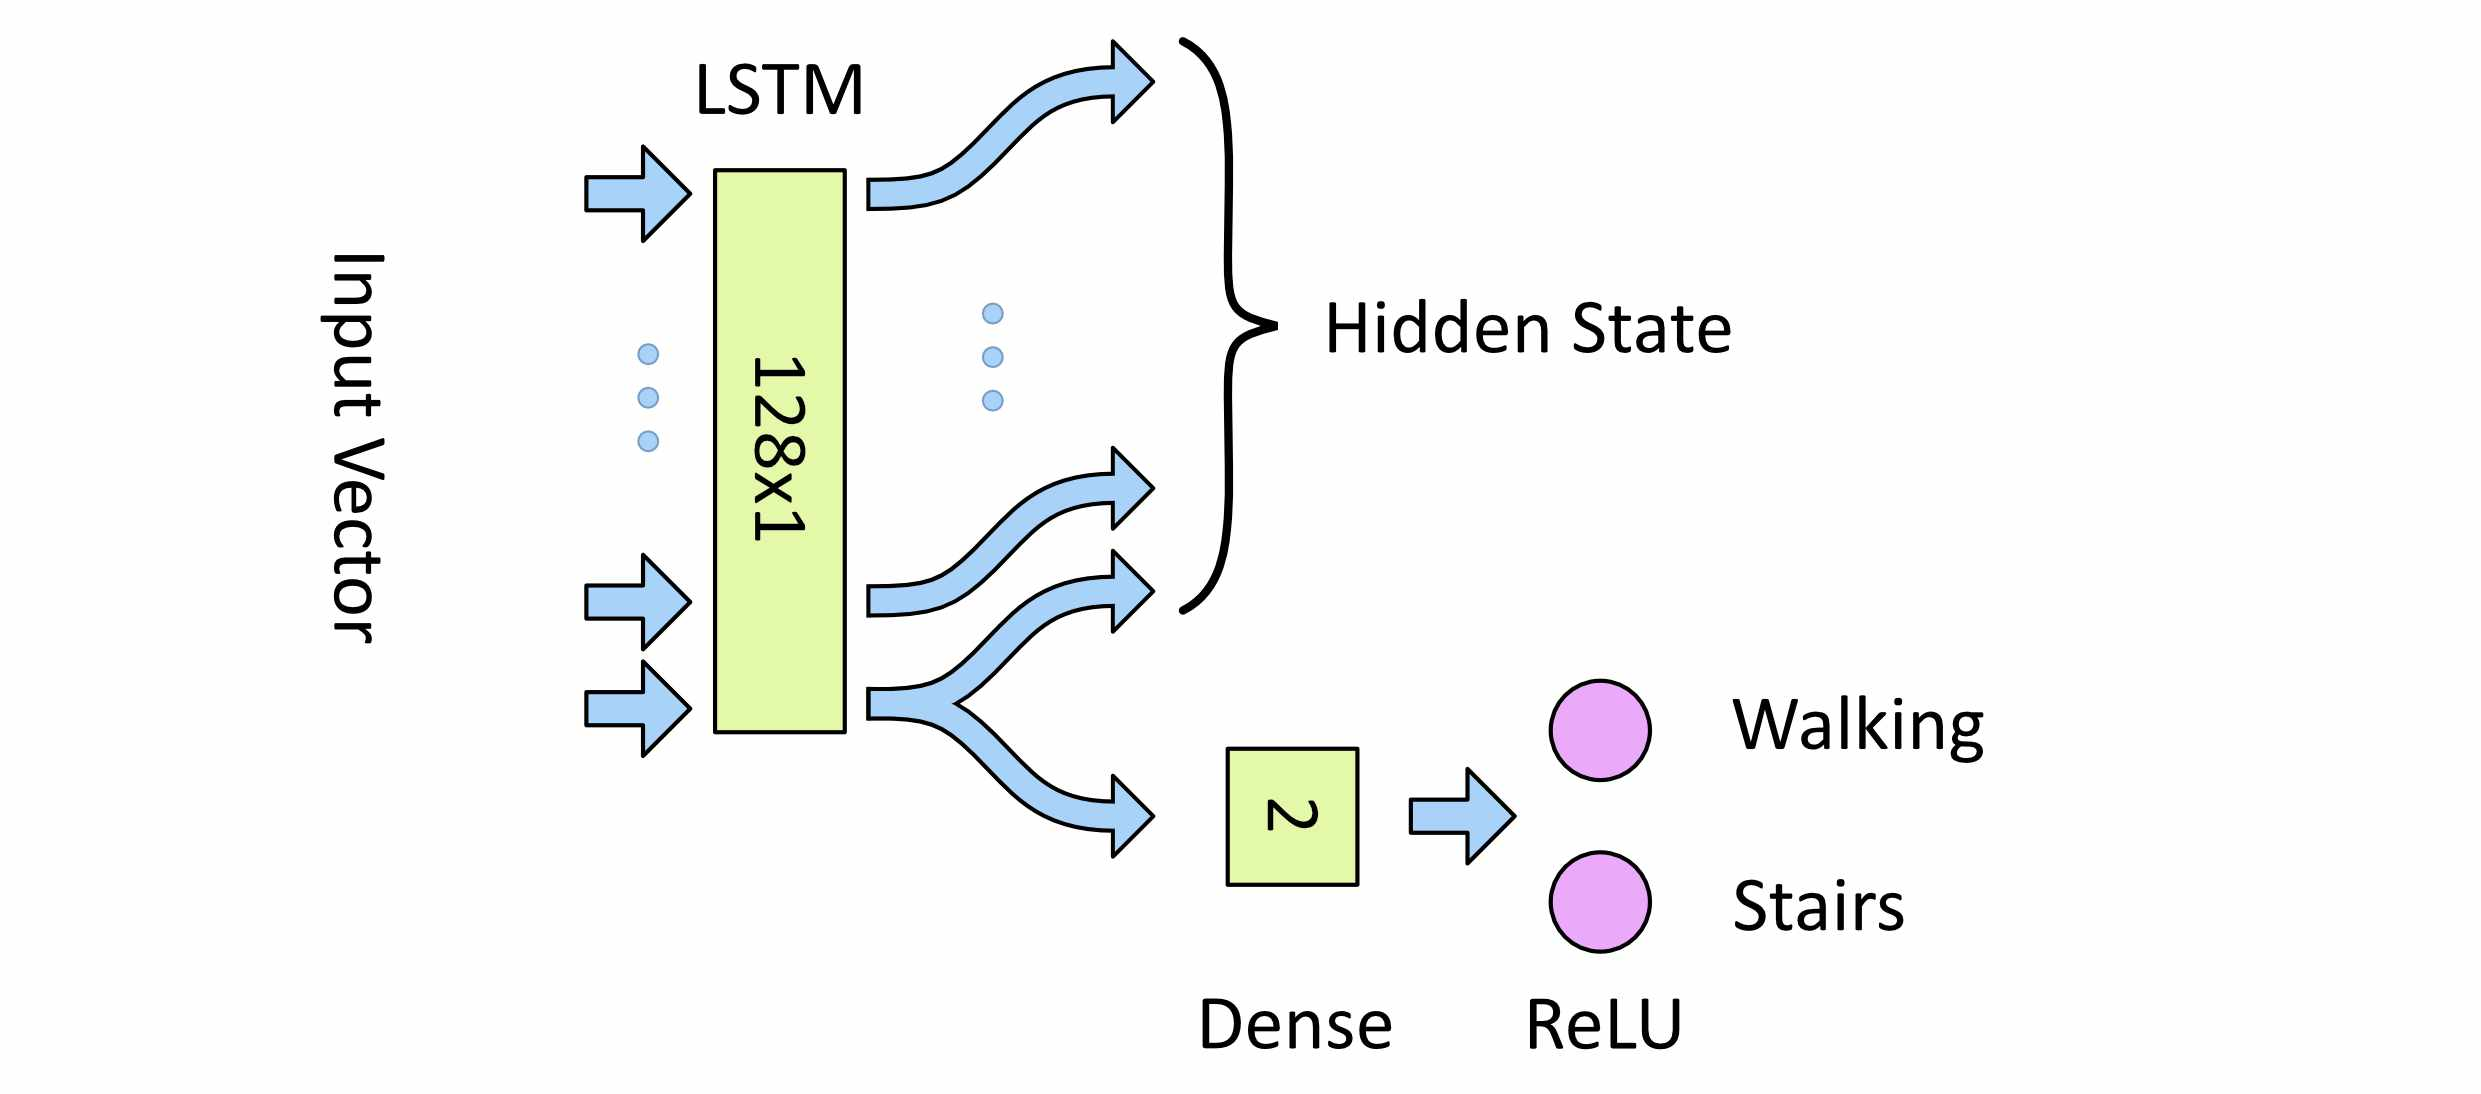
\includegraphics[width=0.8\textwidth]{Figures/lstm/Simplified_Network.jpg}
    \caption{Illustration of simplified model}
    \label{fig:simplfied_lstm_model}
\end{figure}

% How are we simplifying the classification problem so the basic model can solve it
Justification for simplifying the problem. The simple model is not complex enough to solve the full problem, as such in order to get a reasonable classification accuracy the problem needs to be simplified. This simplification can be done either through reducing the number of classes or only training the network to understand certain classes. How are we simplifying the problem? A combination of both will be used, training the model to classify the three most prevalent activities in the data set, W, SA, SD, in different combinations. For example a walking class and a stair class (SA and SD). Why are we only looking at the ankle sensor?

% Analysis methods
To observe the change in information level within network the hidden state value will be used. This will be plotted such that patterns in output for different activities can be seen. To achieve this multiple windows of data will be plotted over top each other all with the same starting point. To account for variation in gait cadence throughout the data set the x axis will be plotted as percentage of gait cycle. Each different activity will be plotted independently. The information gained from these observations will be tested against performance of the full model.

%%%%%%%%%%%%%%%%%%%%%%%%%%%%%%%%%%%%%%%%%%
%%% Results and analysis
\subsection{Results and Analysis}
Within this section the results of the simplified LSTM model are presented. Four different combinations of output class for the activities Walking, Stair Ascent and Stair Descent, were tested as well as four different combinations of input sensor, Y Gyroscope, X Accelerometer, Y Gyro \% X Accel and the full 6 axis IMU. The y gyroscope and x accelerometer were selected as from the previous analysis they showed the greatest variation between subjects.

Table \ref{tab:simplified_model_perfomances} presents the classification accuracies of each input and class combination. For each model classification accuracy was recorded for the validation data and a set of unseen test data from excluded participants. It can be seen that all the models performed equally well for both validation and test data sets. Given the simplicity of the models this suggests that an LSTM is capable of separating the activities from only prominent features.

The models struggled to separate stair descent from the other two activities and, apart from with the 6 axis IMU, most accurately classified stair ascent. From the gait trends this is likely because stair ascent is the most different of the three. All achieved there lowest performance when attempting the hardest task of classifying all three activities individually. An input of the X accelerometer on it's own performed most accurately, even compared to models with multiple input sensors channels. When using only the Y Gyroscope it wasn't possible to separate three activities independently.

\begin{table}[!hbt]
    \centering
    \caption{Summary of simplified model performance}
    \label{tab:simplified_model_perfomances}
    \begin{tabular}{cccc}
        \textbf{Model Classes} & \textbf{Sensor} & \textbf{Validation Accuracy} & \textbf{Test Accuracy}\\
        \hline
        W, SA+SD & Y Gyroscope & 71.6\% & 86.0\% \\
        SA, W+SD & Y Gyroscope & 82.7\% & 83.7\% \\
        SD, W+SA & Y Gyroscope & 57.9\% & 65.6\% \\
        *W, SA, SD & Y Gyroscope & - & - \\
        W, SA+SD & X Accelerometer & 86.6\% & 89.2\% \\
        SA, W+SD & X Accelerometer & 88.6\% & 87.1\% \\
        SD, W+SA & X Accelerometer & 78.4\% & 81.9\% \\
        W, SA, SD & X Accelerometer & 71.9\% & 72.4\%\\
        W, SA+SD & X Accel \& y Gyro & 59.3\% & 48.8\% \\
        SA, W+SD & X Accel \& y Gyro & 71.2\% & 67.1\% \\
        SD, W+SA & X Accel \& y Gyro & 75.1\% & 80.8\% \\
        W, SA, SD & X Accel \& y Gyro & 58.6\% & 66.2\%\\
        W, SA+SD & 6 axis IMU & 82.0\% & 83.3\% \\
        SA, W+SD & 6 axis IMU & 74.2\% & 71.8\% \\
        SD, W+SA & 6 axis IMU & 55.3\% & 63.3\% \\
        W, SA, SD & 6 axis IMU & 48.0\% & 50.7\%\\
        \multicolumn{4}{l}{\footnotesize{* Unable to train a model that could classify this set of classes}}
    \end{tabular}
\end{table}

% \subsection{Hidden State}
Figures \ref{fig:hidden-state-gyro-y-w_v_sa-sd} and \ref{fig:hidden-state-accel-x-w_v_sa-sd} show the trend in hidden state value for a simplified model. In Figure \ref{fig:hidden-state-gyro-y-w_v_sa-sd} the model is classifying stair ascent from a combined class of stair descent and walking. For figure \ref{fig:hidden-state-accel-x-w_v_sa-sd} the model is classifying walking from stairs (ascent and descent). Each of the activities is plotted in a different color, blue solid for walking, green dashed for stair ascent and orange dot dash for stair descent. The five plots each show the hidden state for each timestep with each window starting at the same percentage offset from the beginning of the gait cycle. The x-axis has units of percentage gait cycle, the Y-axis is the dimensionless output of the hidden state. Figure \ref{fig:hidden-state-gyro-y-w_v_sa-sd} has an input of the Y axis gyroscope and \ref{fig:hidden-state-accel-x-w_v_sa-sd} the x accelerometer.

\begin{figure}[!hbt]
     \centering
     \begin{subfigure}[b]{0.32\textwidth}
         \centering
         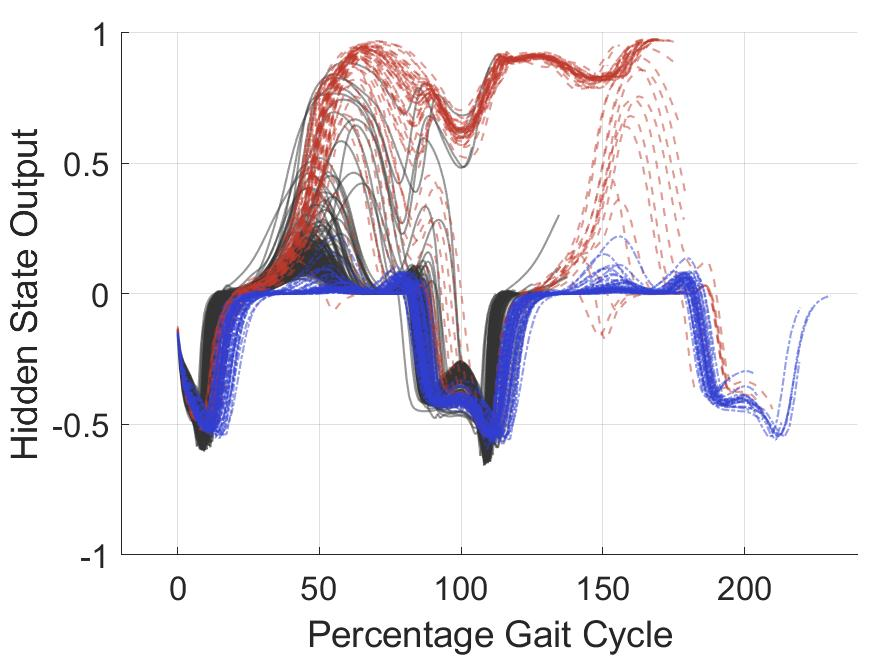
\includegraphics[width=\textwidth]{Figures/results/hidden_state/gyro_y_sa_v_w-sd/0_Participant_04.jpg}
         \caption{0\%}
         \label{subfig:gyro_y_w_v_sa_sd_0}
     \end{subfigure}
     \hfill
     \begin{subfigure}[b]{0.32\textwidth}
         \centering
         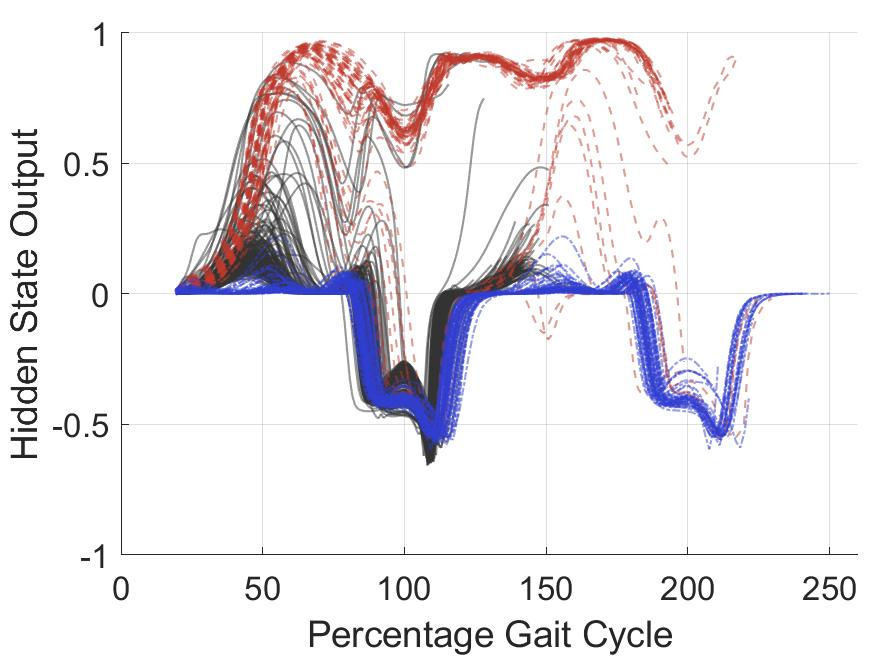
\includegraphics[width=\textwidth]{Figures/results/hidden_state/gyro_y_sa_v_w-sd/20_Participant_04.jpg}
         \caption{20\%}
         \label{subfig:gyro_y_w_v_sa_sd_20}
     \end{subfigure}
     \hfill
     \begin{subfigure}[b]{0.32\textwidth}
         \centering
         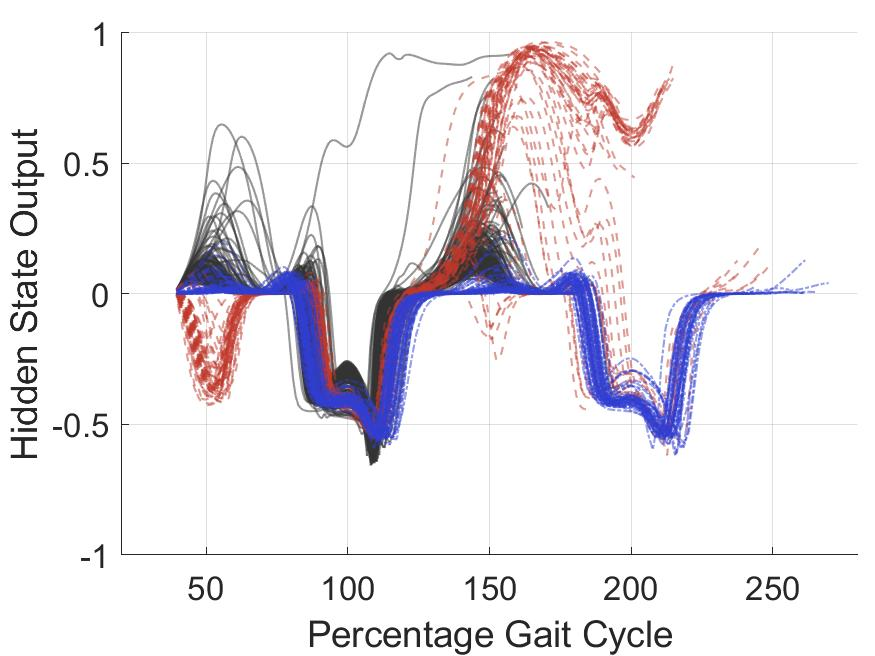
\includegraphics[width=\textwidth]{Figures/results/hidden_state/gyro_y_sa_v_w-sd/40_Participant_04.jpg}
         \caption{40\%}
         \label{subfig:gyro_y_w_v_sa_sd_40}
     \end{subfigure}
     \vskip\baselineskip
     \begin{subfigure}[b]{0.32\textwidth}
         \centering
         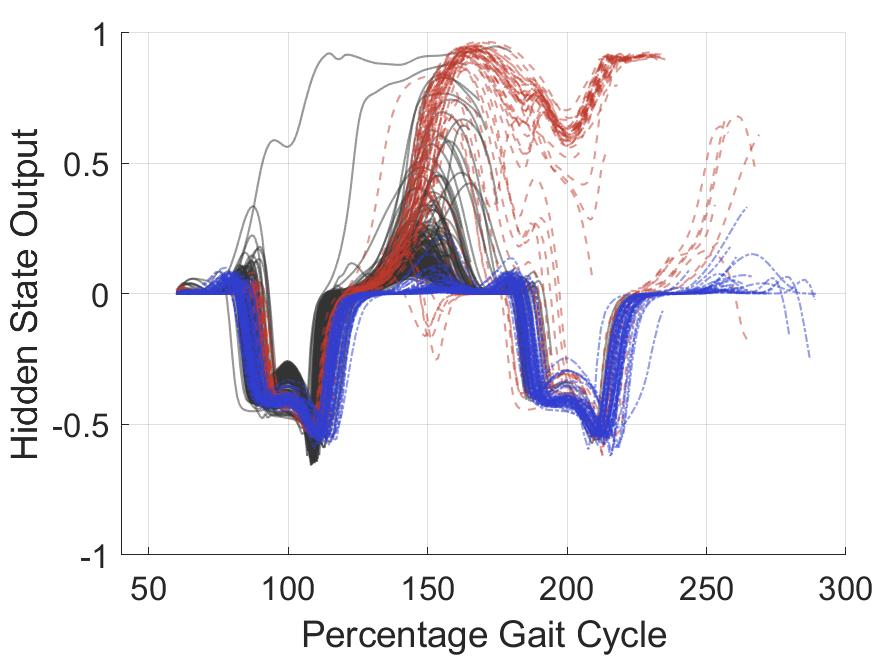
\includegraphics[width=\textwidth]{Figures/results/hidden_state/gyro_y_sa_v_w-sd/60_Participant_04.jpg}
         \caption{60\%}
         \label{subfig:gyro_y_w_v_sa_sd_60}
     \end{subfigure}
     \hspace{0.5em}
     \begin{subfigure}[b]{0.32\textwidth}
         \centering
         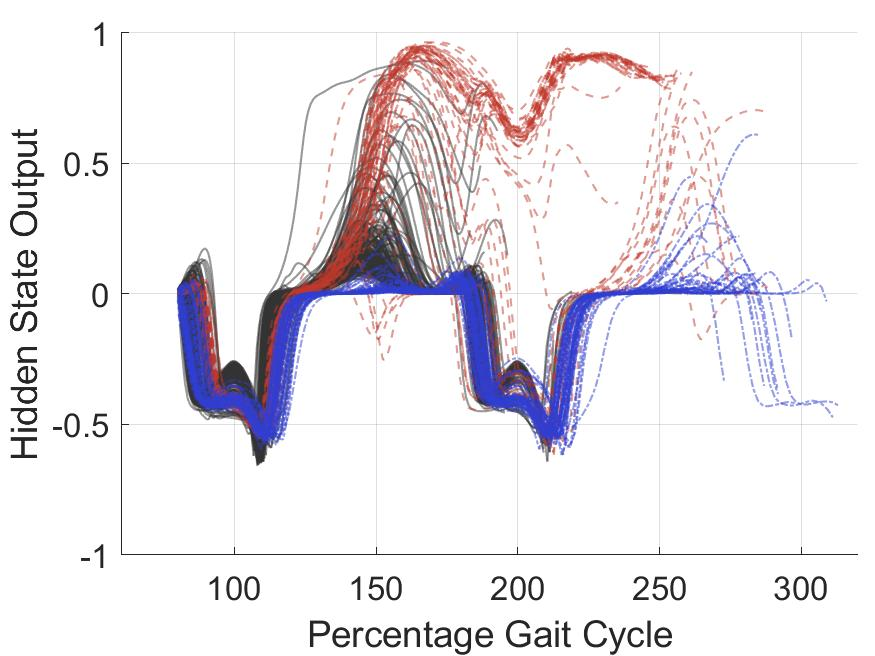
\includegraphics[width=\textwidth]{Figures/results/hidden_state/gyro_y_sa_v_w-sd/80_Participant_04.jpg}
         \caption{80\%}
         \label{subfig:gyro_y_w_v_sa_sd_80}
     \end{subfigure}
    \caption{Hidden state of single unit LSTM model with x axis accelerometer as it's input. The model output classifies stair ascent from walking and stair descent. walking (blue), stair ascent (green) and stair descent (orange)}
    \label{fig:hidden-state-gyro-y-w_v_sa-sd}
\end{figure}

\begin{figure}[!hbt]
     \centering
     \begin{subfigure}[b]{0.32\textwidth}
         \centering
         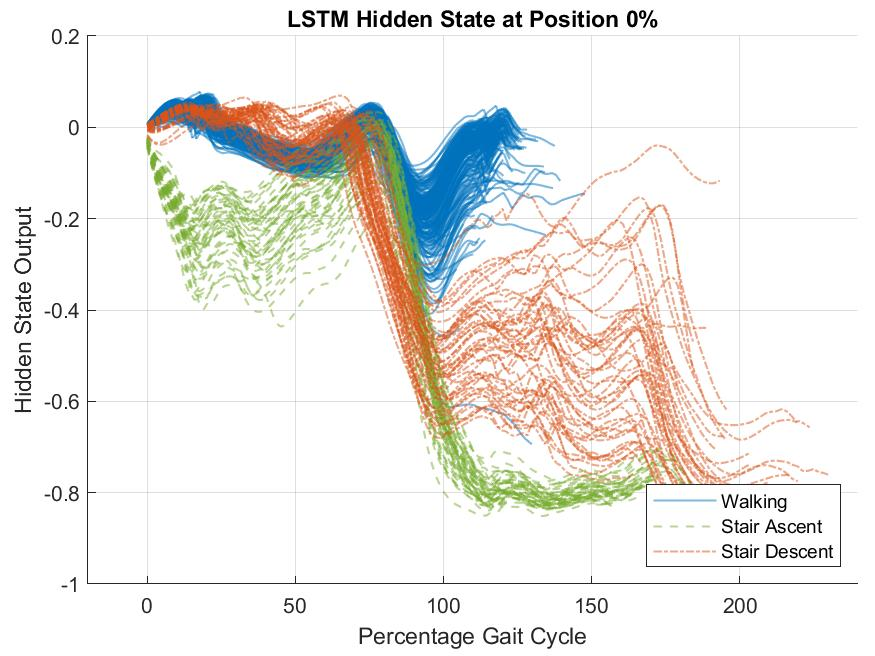
\includegraphics[width=\textwidth]{Figures/results/hidden_state/accel_x_w_v_sa-sd/0_Participant_04.jpg}
         \caption{0\%}
         \label{subfig:a}
     \end{subfigure}
     \hfill
     \begin{subfigure}[b]{0.32\textwidth}
         \centering
         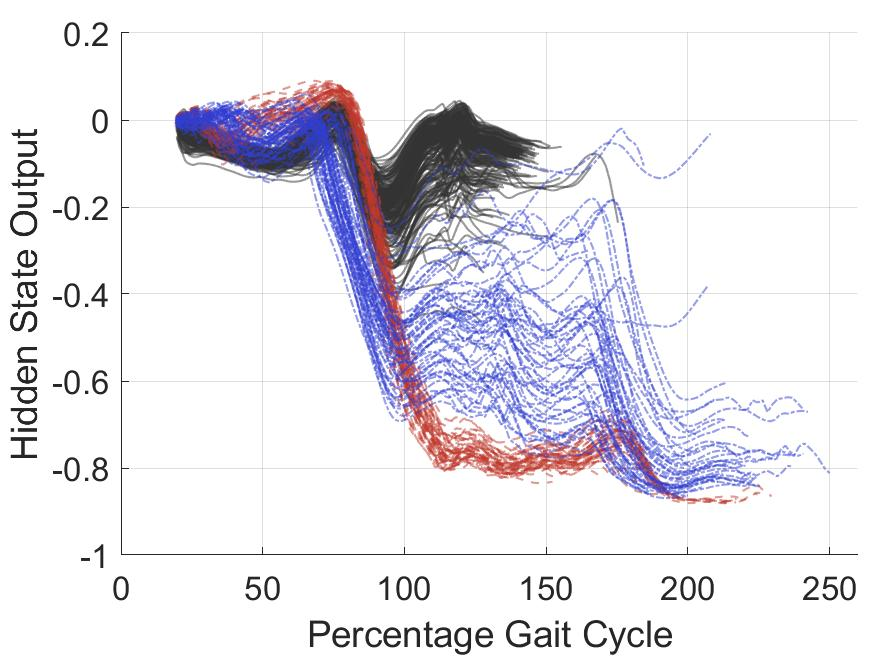
\includegraphics[width=\textwidth]{Figures/results/hidden_state/accel_x_w_v_sa-sd/20_Participant_04.jpg}
         \caption{20\%}
         \label{subfig:b}
     \end{subfigure}
     \hfill
     \begin{subfigure}[b]{0.32\textwidth}
         \centering
         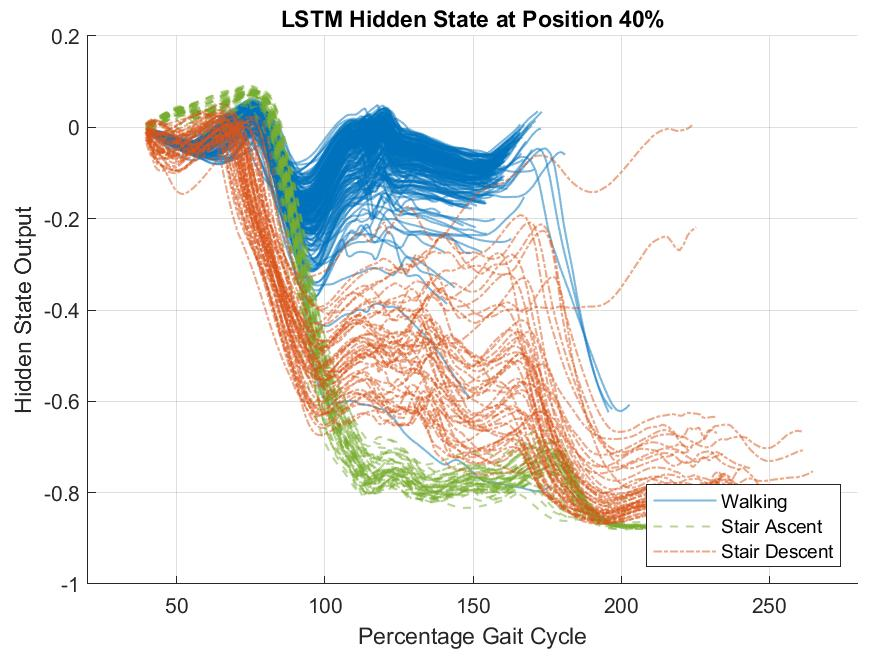
\includegraphics[width=\textwidth]{Figures/results/hidden_state/accel_x_w_v_sa-sd/40_Participant_04.jpg}
         \caption{40\%}
         \label{subfig:c}
     \end{subfigure}
     \vskip\baselineskip
     \begin{subfigure}[b]{0.32\textwidth}
         \centering
         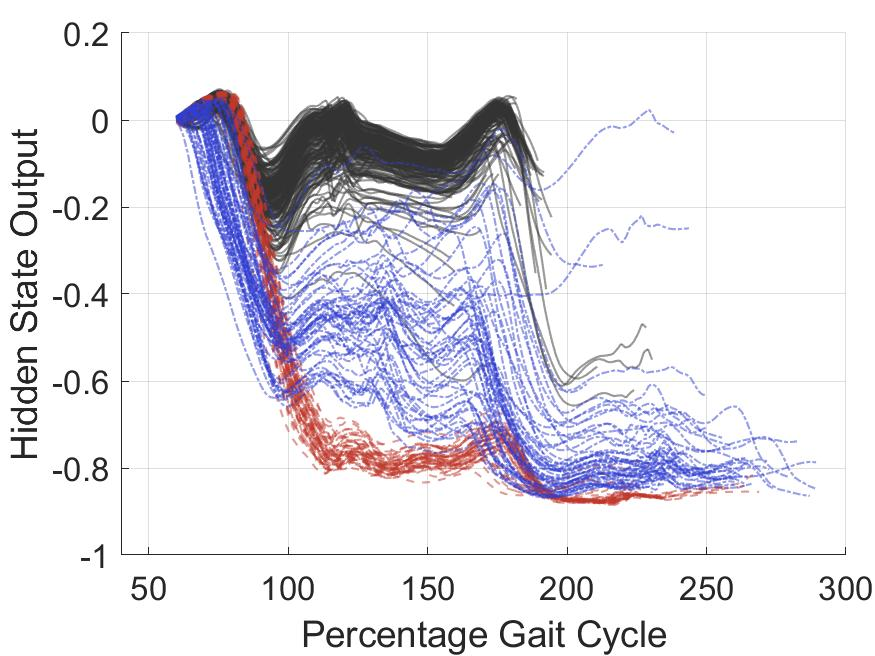
\includegraphics[width=\textwidth]{Figures/results/hidden_state/accel_x_w_v_sa-sd/60_Participant_04.jpg}
         \caption{60\%}
         \label{subfig:d}
     \end{subfigure}
     \hspace{0.5em}
     \begin{subfigure}[b]{0.32\textwidth}
         \centering
         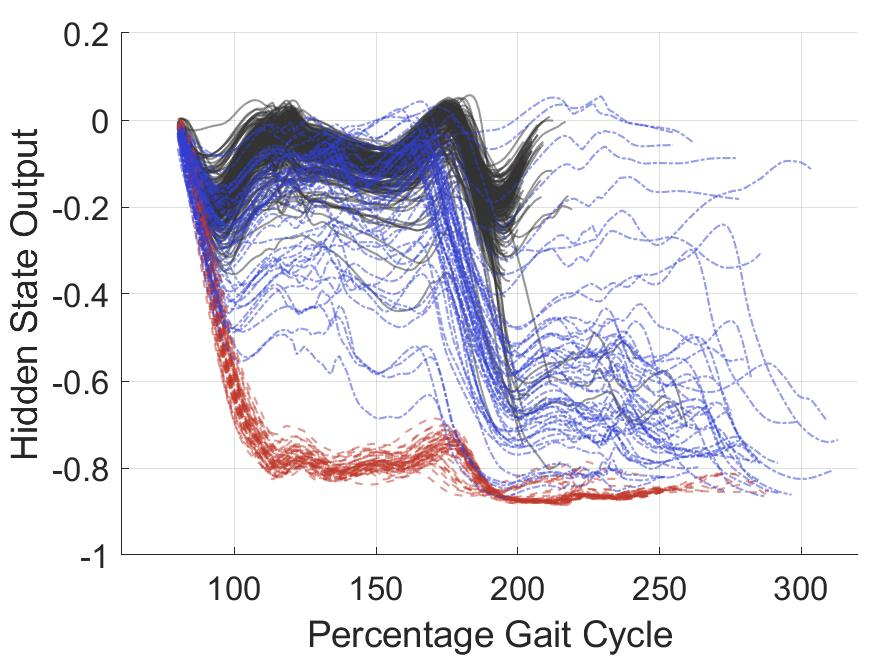
\includegraphics[width=\textwidth]{Figures/results/hidden_state/accel_x_w_v_sa-sd/80_Participant_04.jpg}
         \caption{80\%}
         \label{subfig:e}
     \end{subfigure}
    \caption{Hidden state of single unit LSTM model with x axis accelerometer as it's input. The model output classifies walking from stairs (ascent and stair descent). walking (blue), stair ascent (green) and stair descent (orange)}
    \label{fig:hidden-state-accel-x-w_v_sa-sd}
\end{figure}

For both acceleration and gyroscope the hidden state value changes most during swing and early stance. For the y gyroscope it can be seen that the classification of stair ascent from walking and stair descent occurs around 50\% gait cycle. From the gait trends this is about the point the gyroscope signals begin to converge. 

With the x accelerometer as in input there is less tightly grouped hidden state trends, correlates well with the higher standard deviation. Stair descent is less certain and the model struggles to separate it from walking. Stair ascent and walking are easily classified. Classification occurs around early swing.

No gain from having a window size greater than one step, classification only occurs in one phase of the cycle. It appear that to gain higher accuracy the model would need to learn more personalised information. For both input signals a similar behaviour was observed for all the output class sets.







%%%%%%%%%%%%%%%%%%%%%%%%%%%%%%%%%%%%%%%%%%%%%%%%%%%%%%%%%%%%%%%%%%%%%%%%%%%%
\section{Full Complexity Network}
\label{sec:full_complexity}
% What's in this section
To solve the full problem a more complex model is needed. This will be variations on the architecture presented by Murad et al discussed in \ref{sec:lstm_therory}. Withing this section the effect of hyper-parameters selection on it's performance will be evaluated by parametrically sweeping values. This will allow ideas and observations established from the simplified model to be tested to see if the knowledge is transferable to more complex examples.

For models with fully connected layers the hidden state becomes too convoluted to interpret directly. Model performance will be analysed using percentage classification accuracy, using validation data for trained model performance, and using the unseen test data as a metric for it's generalisation. Confusion matrices will be used to establish how well the model performs per class.

The following hyper-parameters will be investigated:
\begin{itemize}
    \item Window size
    \item LSTM units
    \item Number of layers
    \item Number of inputs - by varying the number of axis and number of sensors
    \item Number of training participants
\end{itemize}

%%%%% Results and analysis
\subsection{Results and Analysis}
The following section presents the results of investigations into how model performance changes with adjustments of hyper-parameters.

For network size three different window sizes (32, 64 and 128 timesteps) and unit widths (4, 6, 8, 16, 32, 64) were tested. Each model shape was trained five times for the five different train/test data sets. Table \ref{tab:model_size_hyper_param} presents the model accuracy achieved for each models $\pm$ standard deviation. Table \ref{tab:model_size_hyper_param_train} and \ref{tab:model_size_hyper_param_test} show the validation and unseen participant test classification accuracy respectively for each configuration.

\begin{table}[!hbt]
    \centering
    \caption{Model accuracy for hyper-parameters for layer units and input window size for both seen and novel subjects}
    \label{tab:model_size_hyper_param}
    \begin{subtable}{.49\linewidth}
        \centering
        \caption{Accuracy for seen validation data}
        \label{tab:model_size_hyper_param_train}
        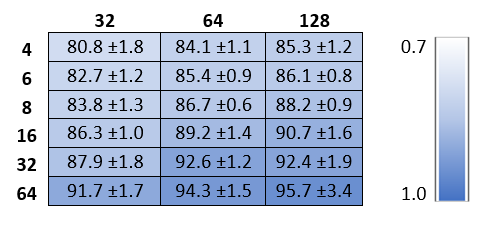
\includegraphics[width=\textwidth]{Figures/results/LSTM_Train_Accuracy.png}
    \end{subtable}
    \hfil
    \begin{subtable}{.49\linewidth}
        \centering
        \caption{Accuracy for unseen test data}
        \label{tab:model_size_hyper_param_test}
        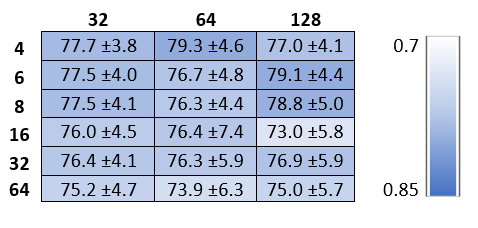
\includegraphics[width=\textwidth]{Figures/results/LSTM_Test_Accuracy.png}
    \end{subtable}
\end{table}

The validation accuracy increases with increasing model size. the improvement when moving from a 32 timestep widow to 64 is much greater than when increasing to 128. For test accuracy the results plateau around 80\%, after which the improvements in performance likely occur due to over fitting to the training data. This also corresponds with an increase in standard deviation.

Networks with two to four deep LSTM layers were tested but this showed no improvement in generalisation and only a small improvement in validation accuracy. The same was observed with multiple sensors there was no additional improvement in generalisation beyond a 6-axis IMU only an improvement in seen data accuracy.

%%%%%%%%%%%%%%%%%%%%%%%%%%%%%%%%%%%%%%%%%%
Figure \ref{fig:subject_num_generalisation} presents the changes in accuracy for varying number of participants used during training. The red line represents the smoothed novel test subject accuracy average for the ten models trained. The blue line represents the same for the training validation data. The solid area represent the standard deviation. Between one and twenty training subjects were used with a single excluded participant used for evaluating unseen data performance. Figure \ref{fig:subject_num_generalisation_64x12} and \ref{fig:subject_num_generalisation_128x6} show the results for a 64 timestep 12 unit and 128 time step 6 unit models respectively.

\begin{figure}[!htb]
    \centering
    \begin{subfigure}[b]{0.49\textwidth}
         \centering
        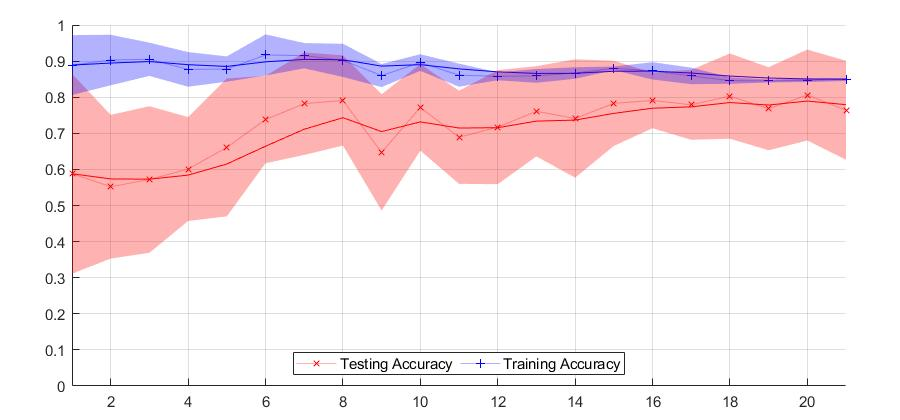
\includegraphics[width=\textwidth]{Figures/results/number_participants_64x12.jpg}
        \caption{64 Timesteps, 12 Units}
        \label{fig:subject_num_generalisation_64x12}
    \end{subfigure}
    \hfil
    \begin{subfigure}[b]{0.49\textwidth}
         \centering
        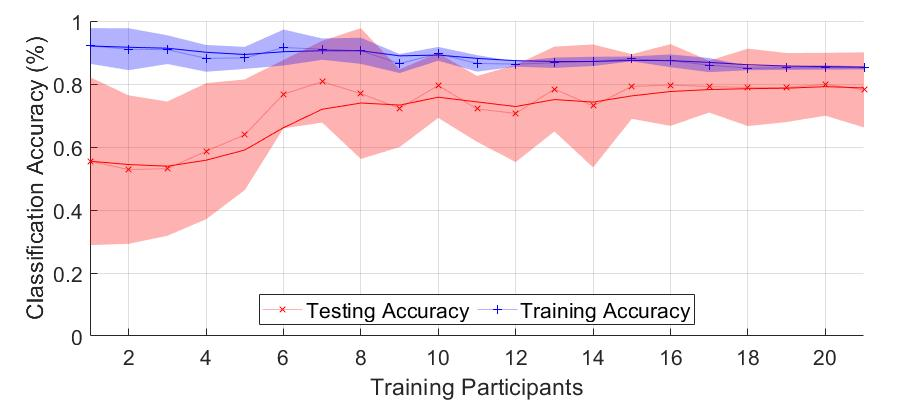
\includegraphics[width=\textwidth]{Figures/results/number_participants_128x6.jpg}
        \caption{128 Timesteps, 6 Units}
        \label{fig:subject_num_generalisation_128x6}
    \end{subfigure}
    \caption{Classification accuracy of seen/unseen subjects for training with different numbers of participants for two different models}
    \label{fig:subject_num_generalisation}
\end{figure}

Figure \ref{fig:subject_num_generalisation} shows that increasing the number of participants leads to better generalised performance, however the effects on increasing numbers of participants levels off around 15 participants. This would indicate that for novel subjects to achieve the high levels of classification performance that are possible with an LSTM increasing the number of subjects alone may not be enough.

%%%%%%%%%%%%%%%%%%%%%%%%%%%%%%%%%%%%%%%%%%
Table \ref{tab:128x6_full_model_confusion_matrix} shows the confusion matrices for a 128 timestep, 6 unit single layer LSTM network. Table \ref{tab:full_model_conf_matrix_training_128x6} is for the training validation data and Table \ref{tab:full_model_conf_matrix_test_128x6} the unseen test data. Table \ref{tab:128x32_full_model_confusion_matrix} shows the same for a model with 32 units. The 6 unit model had a overall classification accuracy of 87.4\% for validation and 84.7\% for test, the 32 unit model accuracy was 96.1\% and 76.0\%.

\begin{table}[!hbt]
    \centering
    \caption{128 timestep, 6 unit confusion matrices}
    \label{tab:128x6_full_model_confusion_matrix}
    \begin{subtable}{.45\textwidth}
        \centering
        \caption{Validation}
        \label{tab:full_model_conf_matrix_training_128x6}
        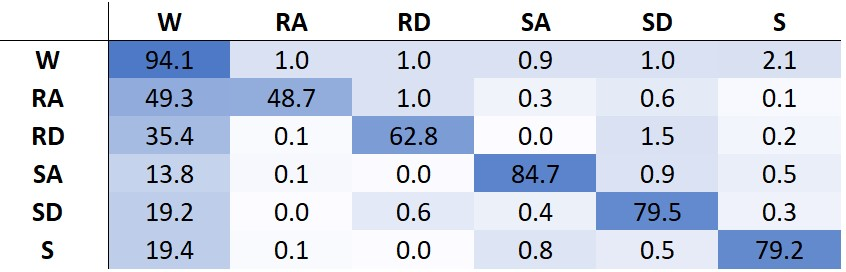
\includegraphics[width=\textwidth]{Figures/results/conf_matricies/Training_128x6_NT.jpg}
    \end{subtable}
    \hfil
    \begin{subtable}{.45\textwidth}
        \centering
        \caption{Test}
        \label{tab:full_model_conf_matrix_test_128x6}
        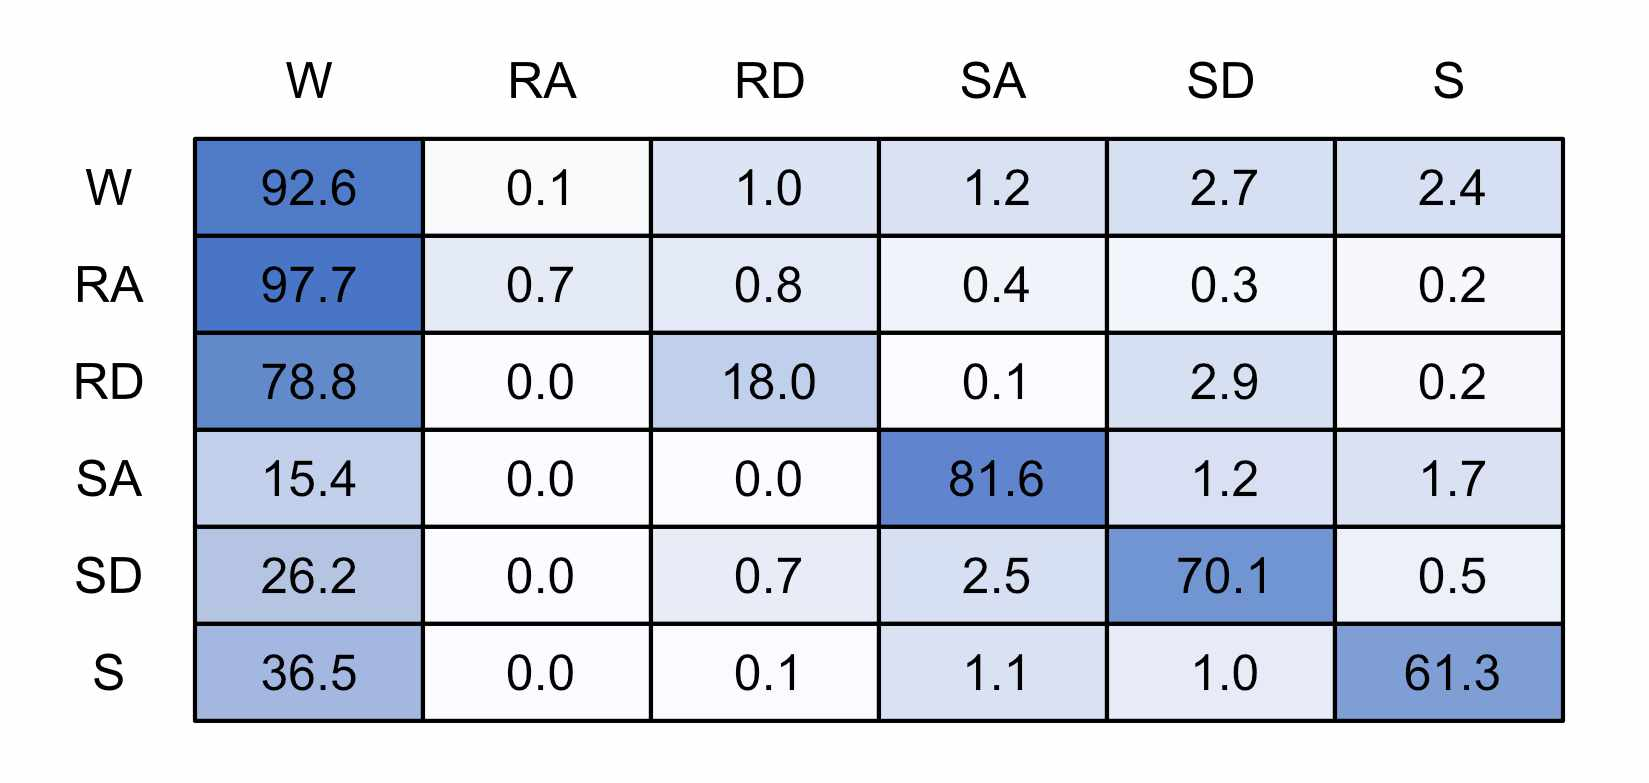
\includegraphics[width=\textwidth]{Figures/results/conf_matricies/Test_128x6_NT.jpg}
    \end{subtable}
\end{table}

\begin{table}[!hbt]
    \centering
    \caption{128 timestep, 32 unit confusion matrices}
    \label{tab:128x32_full_model_confusion_matrix}
    \begin{subtable}{.45\textwidth}
        \centering
        \caption{Validation}
        \label{tab:full_model_conf_matrix_training_128x32}
        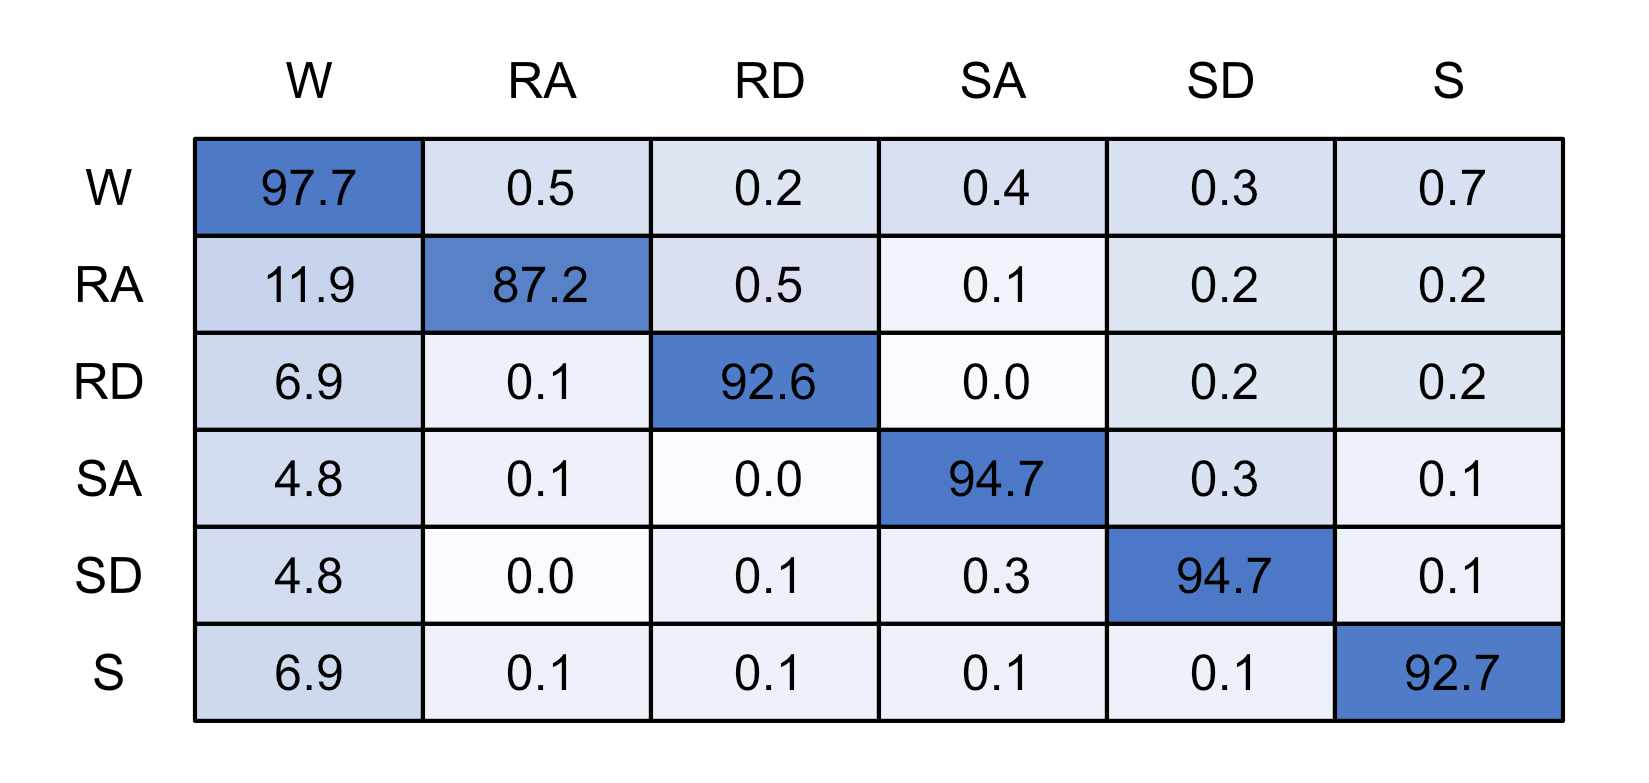
\includegraphics[width=\textwidth]{Figures/results/conf_matricies/Training_128x32_NT.jpg}
    \end{subtable}
    \hfil
    \begin{subtable}{.45\textwidth}
        \centering
        \caption{Test}
        \label{tab:full_model_conf_matrix_test_128x32}
        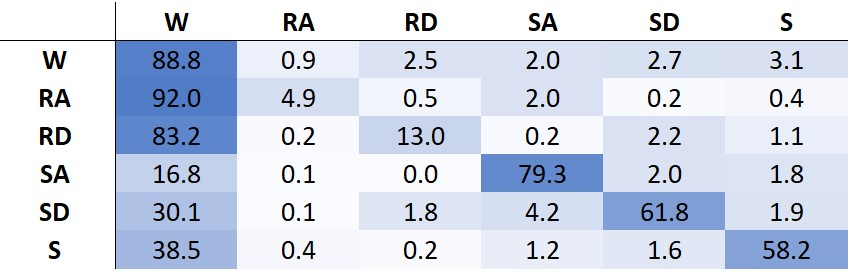
\includegraphics[width=\textwidth]{Figures/results/conf_matricies/Test_128x32_NT.jpg}
    \end{subtable}
\end{table}

It can be seen that nearly all miss-classifications are a confusion with walking. The test data showed a similar patterns for both models even though the 32 unit model is over-fitted to the training data. Some miss-classifications will be due to under labelled or discrepancies in point of labeling during recording.

Ramp descent and ascent the most confused. This is likely because of the similarities in gait cycle between the two activities and the difficulty is accurately labelling this activity due to subject biases on what constitutes a ramp. Stairs get slightly confused between each other but again mostly with walking. Stair Descent performs worse than stair ascent again this is likely due to it's closer gait shape to walking. It's not obvious why stop performs poorly.

%%%%%%%%%%%%%%%%%%%%%%%%%%%%%%%%%%%%%%%%%%
Figure \ref{fig:missclassification} shows a visual representation of the activities labelled during a recording above which is a plot of where the classification errors occur ed during that recording. As can be seen a large proportion of miss-classification occur around changes in activity. The transition between activities is highly varied.

\begin{figure}[!htb]
    \centering
    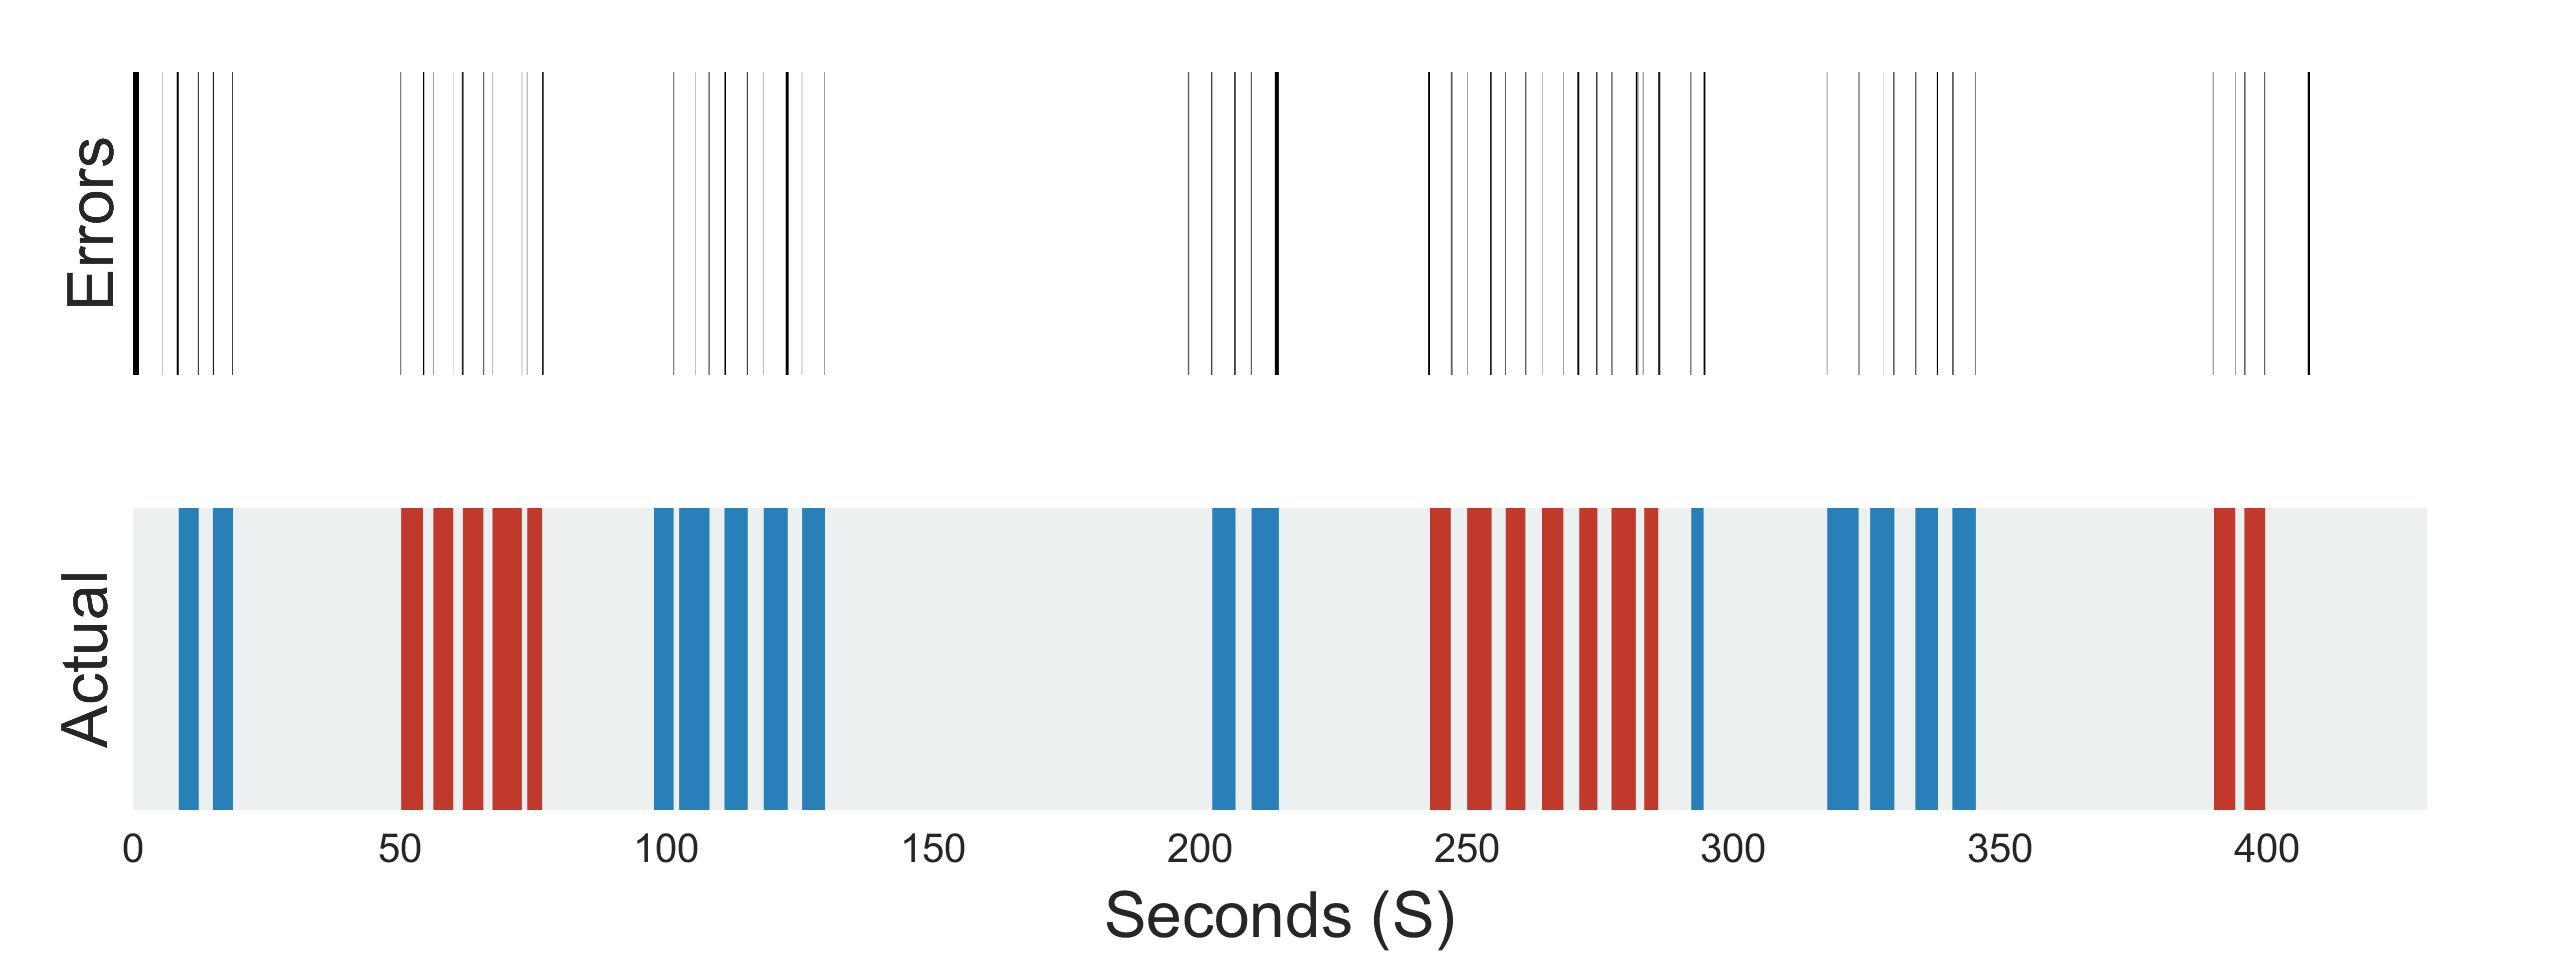
\includegraphics[width=0.8\textwidth]{Figures/results/location_of_errors.jpg}
    \caption{Miss-classifications and labelled activity locations}
    \label{fig:missclassification}
\end{figure}






%%%%%%%%%%%%%%%%%%%%%%%%%%%%%%%%%%%%%%%%%%%%%%%%%%%%%%%%%%%%%%%%%%%%%%
\section{Improving Model Performance}
\label{sec:improving_perfromance} % What were the identified problems above? - Poor generalisation and errors around transition region
%Some kind of introductory paragraph 
From the previous analysis it is clear that the model is not performing well when presented with novel subjects and around changes in activity.
%Demonstration of why individualisation is important and also why it's hard.

\subsection{Individual Gait Patterns}
In order to gauge how different each subject gait is the trends for different activities for each axis were produced. The angular velocity around y and the acceleration in x showed the greatest variation between subjects. Below the trends for these axis for two subject is shown. Figure \ref{fig:imu_gait_trends} shows the mean and standard deviation for three difference activities (W, SA, SD) for two individual subjects. The solid line represents the mean of n gait cycles, and the shaded area the standard deviation. Figures \ref{subfig:x_accel_subj_4} and \ref{subfig:x_accel_subj_16} show the acceleration in the x axis for participants four and sixteen respectively. Figure \ref{subfig:x_gyro_subj_4} and \ref{subfig:x_gyro_subj_16} show the angular velocity in the y axis for the same participants.

\begin{figure}[!htb]
     \centering
     \begin{subfigure}[b]{0.49\textwidth}
         \centering
         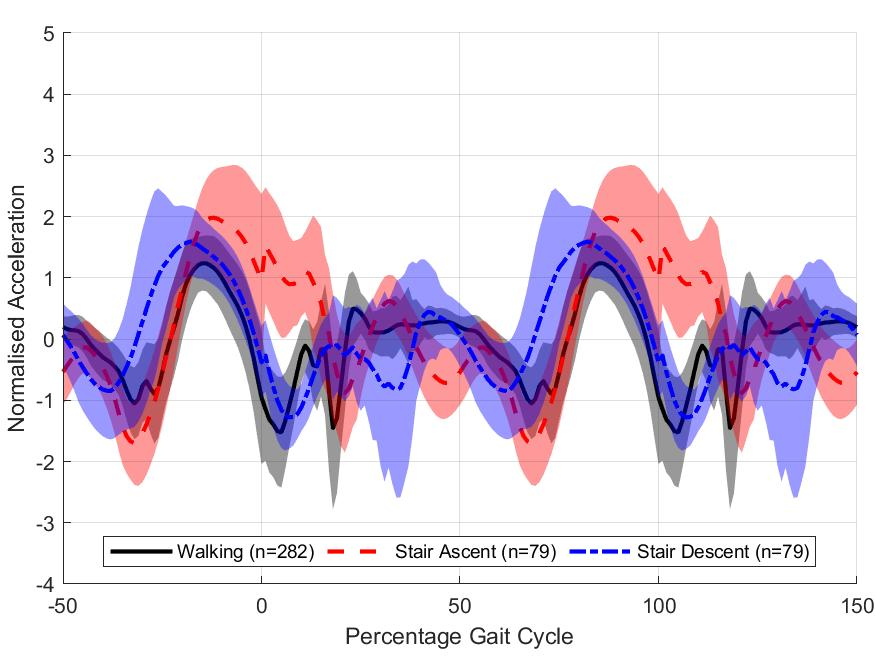
\includegraphics[width=\textwidth]{Figures/gait_trends/accel_x_trend_Participant_04.jpg}
         \caption{Subject 4 - Acceleration in x}
         \label{subfig:x_accel_subj_4}
     \end{subfigure}
     \hfill
     \begin{subfigure}[b]{0.49\textwidth}
         \centering
         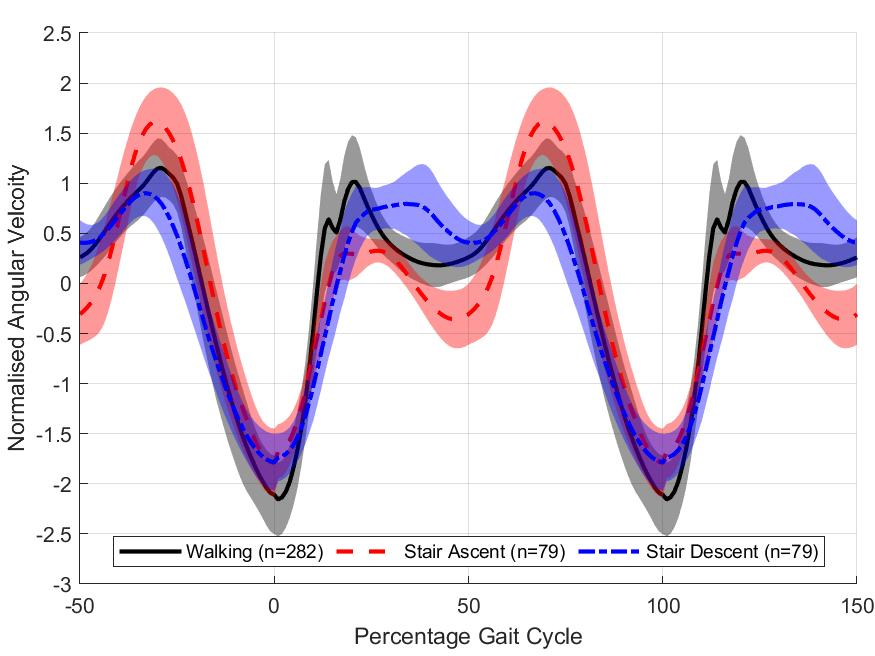
\includegraphics[width=\textwidth]{Figures/gait_trends/gyro_y_trend_Participant_04.jpg}
         \caption{Subject 4 - Shank angular velocity about y}
         \label{subfig:x_gyro_subj_4}
     \end{subfigure}
     \vskip\baselineskip
     \begin{subfigure}[b]{0.49\textwidth}
         \centering
         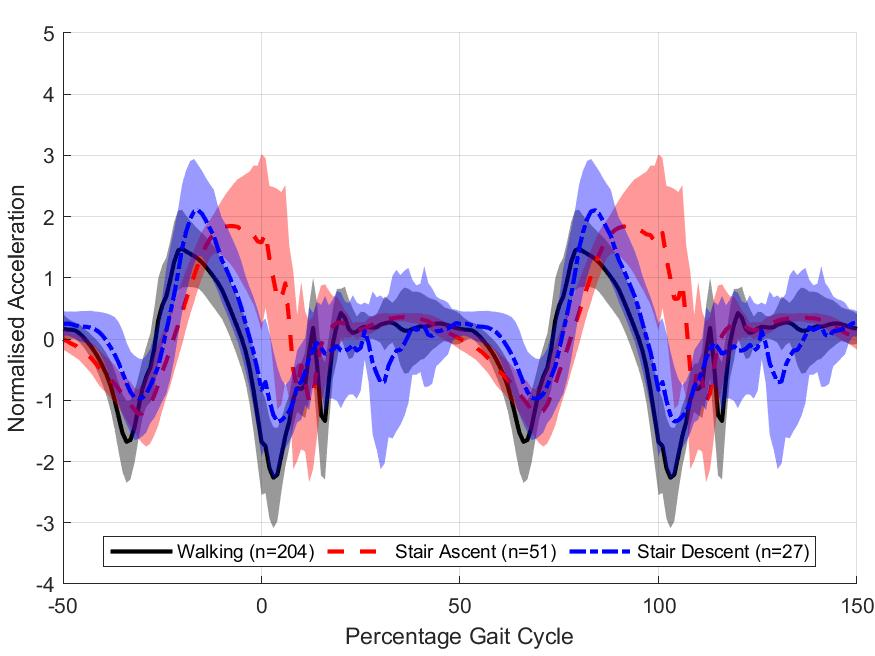
\includegraphics[width=\textwidth]{Figures/gait_trends/accel_x_trend_Participant_16.jpg}
         \caption{Subject 16 - Shank acceleration in x}
         \label{subfig:x_accel_subj_16}
     \end{subfigure}
     \hfill
     \begin{subfigure}[b]{0.49\textwidth}
         \centering
         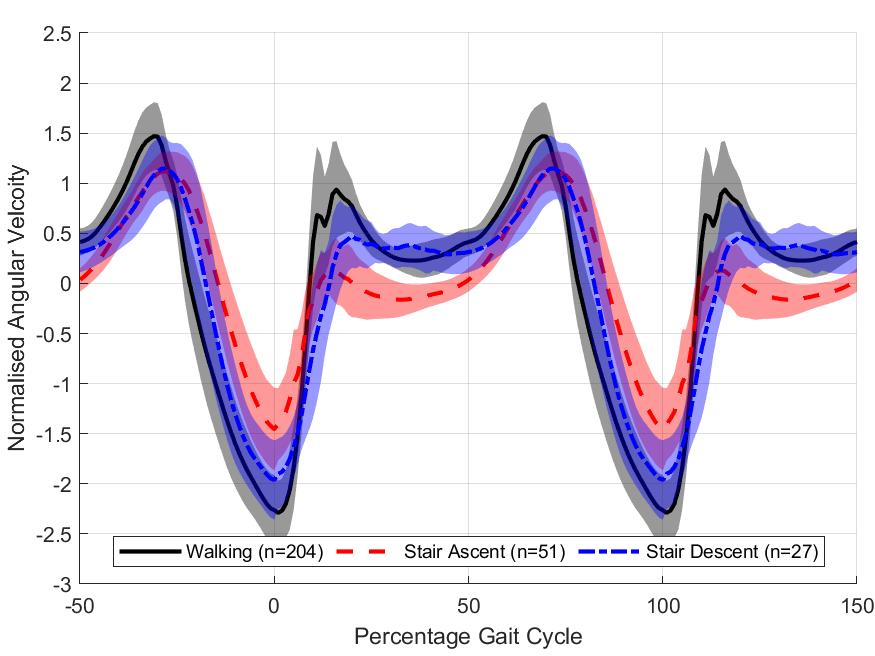
\includegraphics[width=\textwidth]{Figures/gait_trends/gyro_y_trend_Participant_16.jpg}
         \caption{Subject 16 - Shank angular velocity about y axis}
         \label{subfig:x_gyro_subj_16}
     \end{subfigure}
    \caption{Gait trends of two subject for 3 different activities. The solid lines show the mean value for n steps, the shaded area shows the standard deviation. Black solid - Walking, Red dashed - Stair Ascent, Blue dot dash - Stair Descent}
    \label{fig:imu_gait_trends}
\end{figure}

From Figure \ref{fig:imu_gait_trends} the differences between the two chosen participants can be seen. The x acceleration signal is very noisy, with large standard deviation particularly around heel strike, ~20\% gait cycle. For stair ascent there is a delayed peak acceleration with stair descent and walking having very similar shapes.

As explained previously 0\% gait cycle corresponds with the peak y axis shank angular velocity. The maxima following this is a pseudo point for heel strike and the maxima prior for toe off. As expected stair descent results in a large early stance angular velocity and stair ascent a decrease. The difference in peak angular velocity between participants likely a result of climbing stairs at a slower cadence.

The graphs are largely similar, this holds true for the other subjects not shown here, with early stance having the greatest difference between participants for both acceleration and angular velocity. This appears to be the area with greatest information about locomotion mode so may cause issues when generalising.


\subsection{Transition State}
To try and improve this an additional transition state was added to the model
% Methodology
The transition state was added to the classification output and the label data augmented with a transition region added for 0.5 seconds before and after changes in activity. A model was then trained again using the excluded participant cross validation to establish generalisation performance. Two model were trained with 128 time steps and 6 and 32 unit.

% Results
Tables \ref{tab:128x6_transition_confusion_matrix} and \ref{tab:128x32_transition_confusion_matrix} present the confusion matrices for the transition models trained with 6 and 32 units respectively. The 6 unit model achieved 82.8\% accuracy on validation data and 72.4\% for test, and the 32 unit model achieved 93.1\% and 69.3\%. If the transition state is excluded from the classification accuracy then when presented with test data the models achieve 75.2\% and 75.0\% accuracy for the 6 and 32 unit models respectively

\begin{table}[!hbt]
    \centering
    \caption{128x6 Transition Model}
    \label{tab:128x6_transition_confusion_matrix}
    \begin{subtable}{.45\textwidth}
        \centering
        \caption{Training}
        \label{tab:tran_model_conf_matrix_training_128x6}
        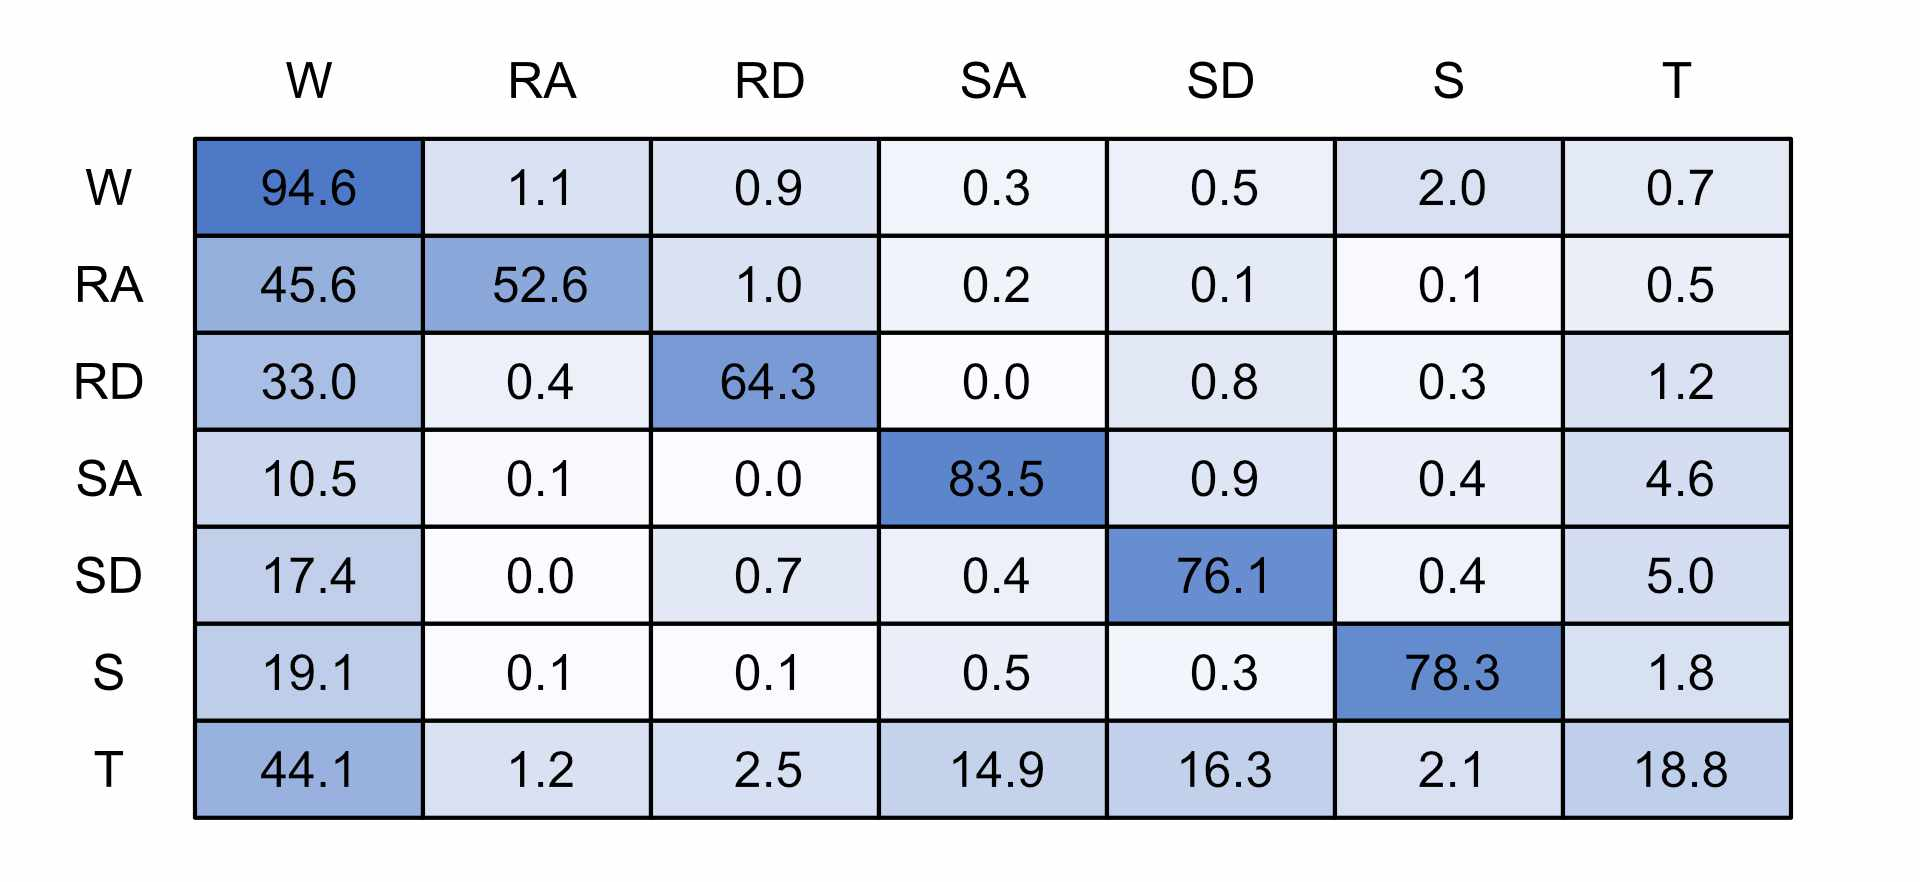
\includegraphics[width=\textwidth]{Figures/results/conf_matricies/Training_128x6_T.jpg}
    \end{subtable}
    \hfil
    \begin{subtable}{.45\textwidth}
        \centering
        \caption{Test}
        \label{tab:tran_model_conf_matrix_test_128x6}
        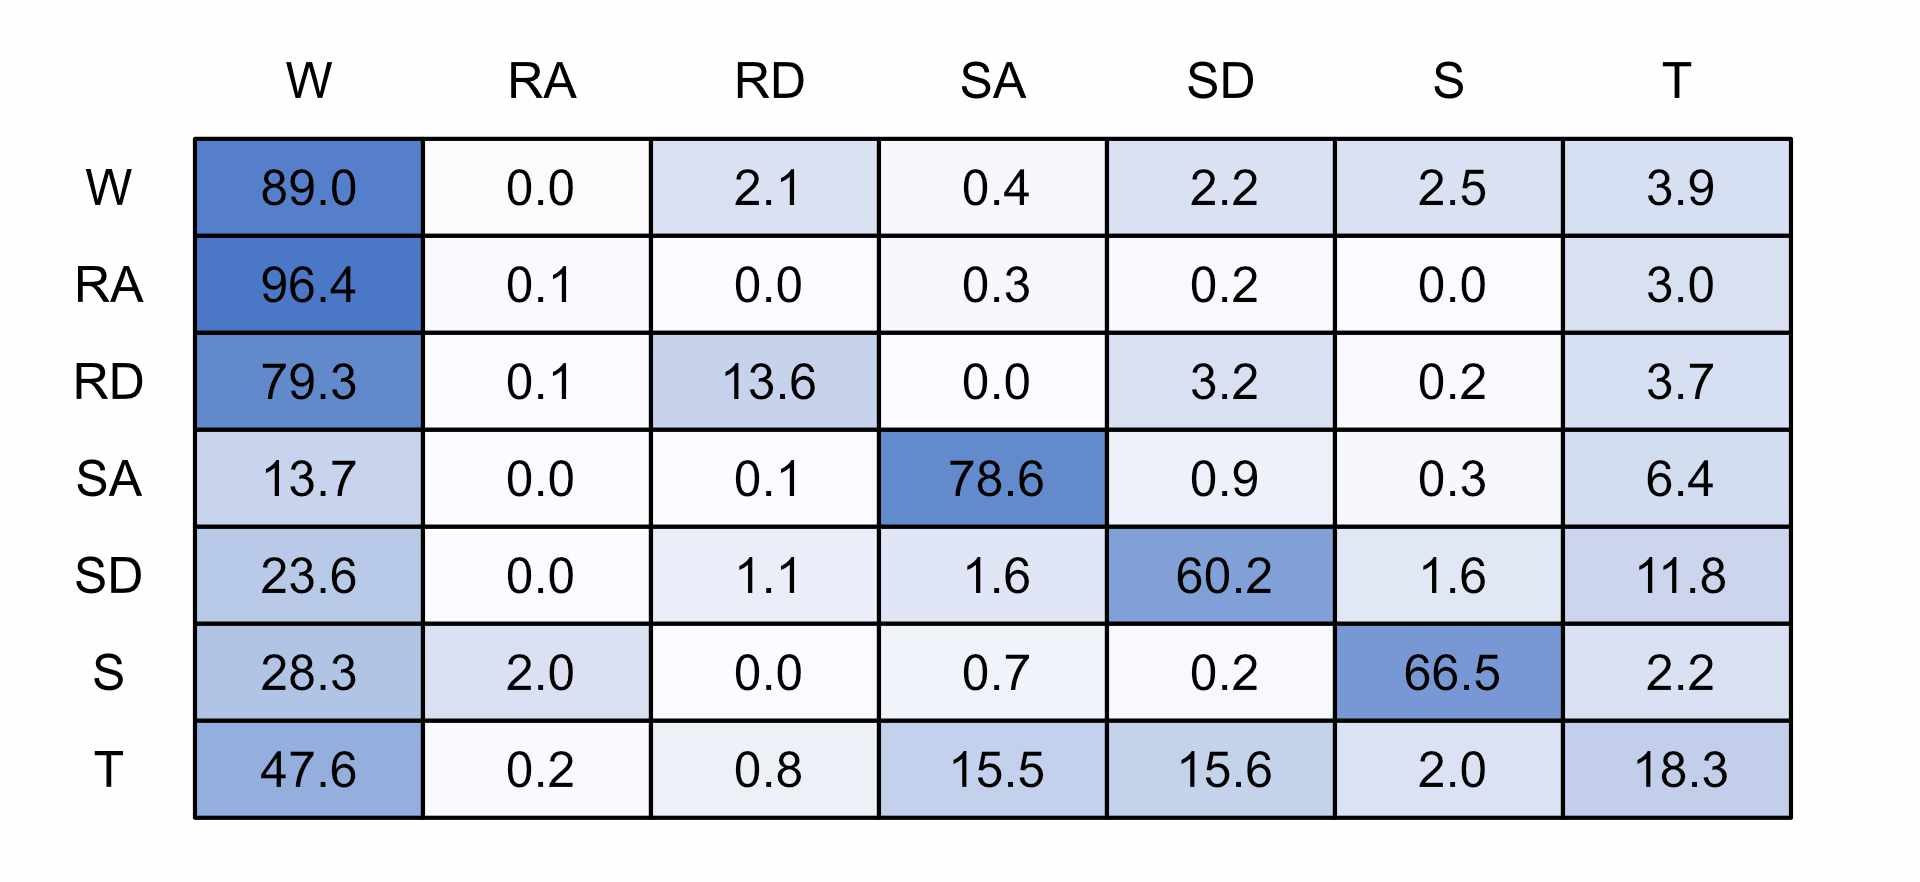
\includegraphics[width=\textwidth]{Figures/results/conf_matricies/Test_128x6_T.jpg}
    \end{subtable}
\end{table}

\begin{table}[!hbt]
    \centering
    \caption{128x32 Transition Model}
    \label{tab:128x32_transition_confusion_matrix}
    \begin{subtable}{.45\textwidth}
        \centering
        \caption{Training}
        \label{tab:tran_model_conf_matrix_training_128x32}
        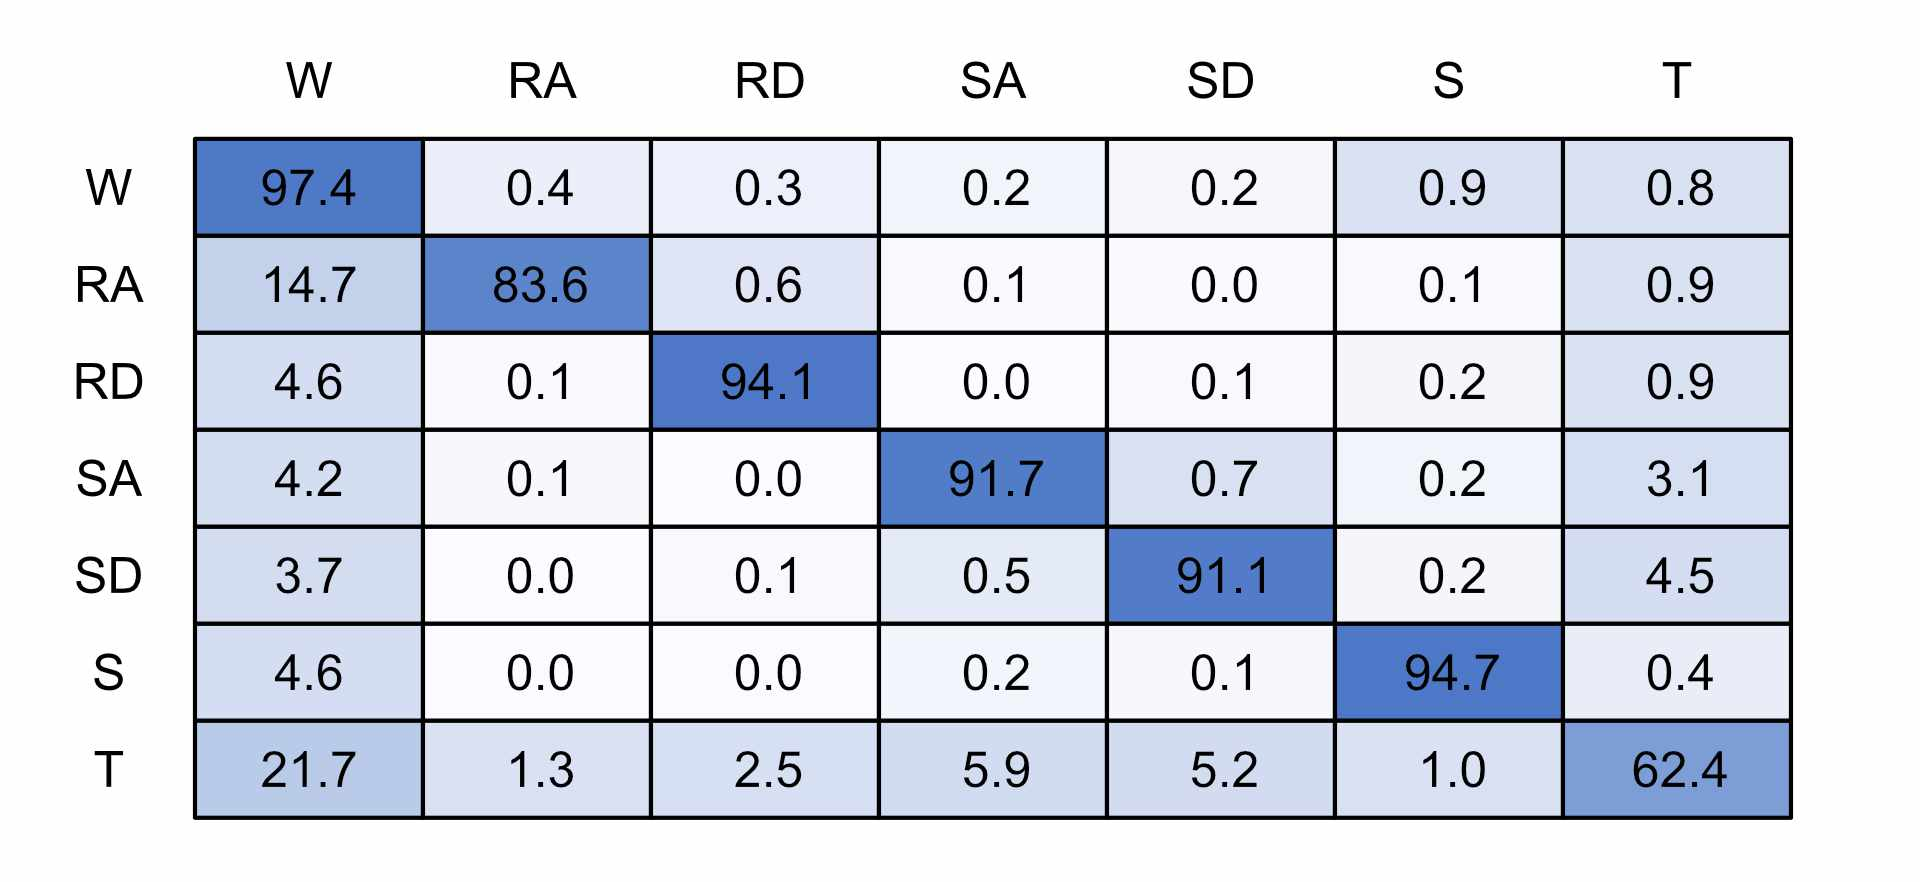
\includegraphics[width=\textwidth]{Figures/results/conf_matricies/Training_128x32_T.jpg}
    \end{subtable}
    \hfil
    \begin{subtable}{.45\textwidth}
        \centering
        \caption{Test}
        \label{tab:tran_model_conf_matrix_test_128x32}
        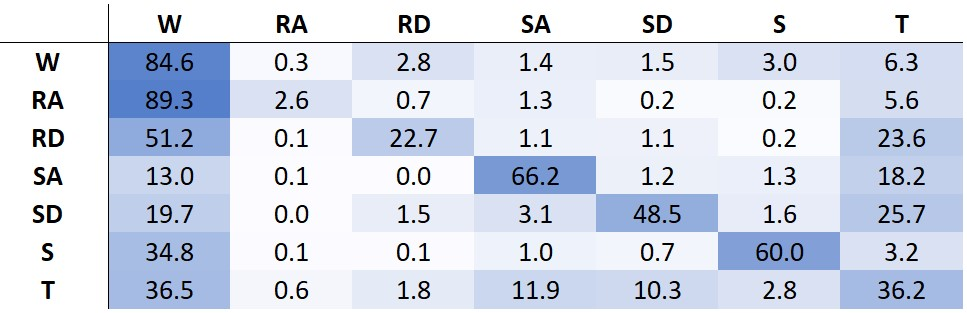
\includegraphics[width=\textwidth]{Figures/results/conf_matricies/Test_128x32_T.jpg}
    \end{subtable}
\end{table}

% Analysis
This method did not improve performance, equal or worse performance than without the transition state, even when excluding the transition state for classification accuracy. The transition region is highly uncertain and so the model will struggle to learn the expected behaviour.

%%%%%%%%%%%%%%%%%%%%%%%%%%%%%%%%%%%%%%%%%%
\section{Discussion}
\label{sec:discussion}
%What did we learn from the simplified model and how was it useful in the full model?
The simplified model gave an insight into which areas of the gait cycle to model is likely to learn. The observations made from this appear to match up well with the larger model performance. Window size doesn't affect performance, as long as the window cover the stance phase the simplified model was able to identify the class. Therefore a window size of greater than one gait cycle offers no benefit as the last stance phase observed sets the final output. As was seen increasing subjects would not necessarily lead to a model that could generalise well to novel subject. As amputees have gaits that are much more varied between individuals this is significantly less likely to work.

The simplified model achieves high accuracy despite it's limited learning ability, albeit on a simplified problem. Therefore the higher accuracy achieved on the full model may in part be by learning the minute personal trends of the data for the participants. This may explain why the models struggle to generalise for new participants unless the model has been trained on a person with similar gait. 85\% appears to be an upper bound for LSTM using just IMU data when presenting novel users, instead of as Dehghani et al stated and over estimation of performance.

It was not really obvious why such deep models have been used in literature and they seem to offer negligible improvements in performance versus there size and result it models that very easily over fit.

The results of this work suggest that simply modifying adjusting the LSTM model hyper-parameters is not enough to produce a model that performs well with unseen users. Alternative approaches are therefore required to solve this problem. Additions to the output such smoothing to combine multiple classifications. Or more complex classifiers where more than just the maximum output value is used, instead classes are used establish how confident the model is. A system of personalisation could also be developed to adapt the model to an individual. It would be of interest to established whether a model trained from able-bodied users could be adapted to lower limb amputees.

%%%%%%%%%%%%%%%%%%%%%%%%%%%%%%%%%%%%%%%%%%
\section{Conclusions}
\label{sec:conclusion}

In this paper, we have presented a new data set for HAR research that...

We have investigated the behaviour of an LSTM using able-bodied subjects to provide suitable quantities of data. We have demonstrated that the learning is applicable to more complex models

Attempted to improve novel user performance by accounting for transitions between activities

Further work is still required in the areas
%Collect more data
%Investigate personalisation techniques
%Apply to amputee

%%%%%%%%%%%%%%%%%%%%%%%%%%%%%%%%%%%%%%%%%%
\vspace{6pt} 


%%%%%%%%%%%%%%%%%%%%%%%%%%%%%%%%%%%%%%%%%%
\authorcontributions{For research articles with several authors, a short paragraph specifying their individual contributions must be provided. The following statements should be used ``conceptualization, X.X. and Y.Y.; methodology, X.X.; software, X.X.; validation, X.X., Y.Y. and Z.Z.; formal analysis, X.X.; investigation, X.X.; resources, X.X.; data curation, X.X.; writing--original draft preparation, X.X.; writing--review and editing, X.X.; visualization, X.X.; supervision, X.X.; project administration, X.X.; funding acquisition, Y.Y.'', please turn to the  \href{http://img.mdpi.org/data/contributor-role-instruction.pdf}{CRediT taxonomy} for the term explanation. Authorship must be limited to those who have contributed substantially to the work reported.}

%%%%%%%%%%%%%%%%%%%%%%%%%%%%%%%%%%%%%%%%%%
\funding{This research was funded by an EPSRC Studentship}
% \funding{Please add: ``This research received no external funding'' or ``This research was funded by NAME OF FUNDER grant number XXX.'' and  and ``The APC was funded by XXX''. Check carefully that the details given are accurate and use the standard spelling of funding agency names at \url{https://search.crossref.org/funding}, any errors may affect your future funding.}

%%%%%%%%%%%%%%%%%%%%%%%%%%%%%%%%%%%%%%%%%%
\acknowledgments{In this section you can acknowledge any support given which is not covered by the author contribution or funding sections. This may include administrative and technical support, or donations in kind (e.g., materials used for experiments).} % Richard Tucker of Amphibian Technologies Limited for loan of the Movesense sensors and programming equipment.

%%%%%%%%%%%%%%%%%%%%%%%%%%%%%%%%%%%%%%%%%%
\conflictsofinterest{The authors declare no conflict of interest. The funders had no role in the design of the study; in the collection, analyses, or interpretation of data; in the writing of the manuscript, or in the decision to publish the results.} 

%%%%%%%%%%%%%%%%%%%%%%%%%%%%%%%%%%%%%%%%%%
%% optional
\abbreviations{The following abbreviations are used in this manuscript:\\
\noindent 
\begin{tabular}{@{}ll}
ADL & Activities of Daily Living\\
BLE & Bluetooth Low Energy \\
HS & Heel Strike \\
HAR & Human Activity Recognition \\
IC & Initial Contact \\
IMU & Inertial Measurement Unit \\
MARG & Magnetic Angular and Rate Gyroscope \\
ML & Machine Learning \\
LOOXV & Leave One Out Cross Validation \\
LSTM & Long Short Term Memory \\
RA & Ramp Ascent \\
RD & Ramp Descent \\
RNN & Recurrent Neural Network \\
PK & Peak Swing \\
S & Stop \\
SA & Stair Ascent \\
SD & Stair Descent \\
TO & Toe Off \\
W & Walking \\
\end{tabular}
}

%%%%%%%%%%%%%%%%%%%%%%%%%%%%%%%%%%%%%%%%%%
%% optional
%%%%%%%%%%%%%%%%%%%%%%%%%%%%%%%%%%%%%%%%%%
% Citations and References in Supplementary files are permitted provided that they also appear in the reference list here. 

%=====================================
% References, variant B: external bibliography
%=====================================
\reftitle{References}
\externalbibliography{yes}
\bibliography{references}

%%%%%%%%%%%%%%%%%%%%%%%%%%%%%%%%%%%%%%%%%%
%% optional
%% for journal Sci
%\reviewreports{\\
%Reviewer 1 comments and authors’ response\\
%Reviewer 2 comments and authors’ response\\
%Reviewer 3 comments and authors’ response
%}

%%%%%%%%%%%%%%%%%%%%%%%%%%%%%%%%%%%%%%%%%%
\end{document}

